\documentclass[
	% -- opções da classe memoir --
	12pt,				% tamanho da fonte
	openright,			% capítulos começam em pág ímpar (insere página vazia caso preciso)
	oneside,			% para impressão em um lado. Oposto a twoside, verso e anverso
	a4paper,			% tamanho do papel. 
	% -- opções da classe abntex2 --
	chapter=TITLE,		% títulos de capítulos convertidos em letras maiúsculas
	section=TITLE,		% títulos de seções convertidos em letras maiúsculas
	%subsection=TITLE,	% títulos de subseções convertidos em letras maiúsculas
	%subsubsection=TITLE,% títulos de subsubseções convertidos em letras maiúsculas
	% -- opções do pacote babel --
	english,			% idioma adicional para hifenização
	%french,				% idioma adicional para hifenização
	%spanish,			% idioma adicional para hifenização
	brazil,				% o último idioma é o principal do documento    
	]{styles/abntex2}

\usepackage[alf]{styles/abntex2cite}	% Citações padrão ABNT
\usepackage[utf8]{inputenc}

\usepackage{lastpage}
\usepackage{times}
\usepackage{soulutf8}
\usepackage{graphicx}
\usepackage{subcaption}
\usepackage{tabularx}
\usepackage{caption}
\captionsetup{justification = raggedright, singlelinecheck = false}

\newcommand{\Fonte}[1]{
    \RaggedRight
    Fonte: #1
}

\usepackage{styles/ttc_univali}
\newcolumntype{Y}{>{\centering\arraybackslash}X}

\title{TTC}
\author{Fernando Concatto}
\date{November 2018}

% make emph bold instead of italic
\let\emph\relax % there's no \RedeclareTextFontCommand
\DeclareTextFontCommand{\emph}{\bfseries}


\begin{document}

\pretextual

\begin{Info}
% Universidade
{UNIVERSIDADE DO VALE DO ITAJAÍ}
% Escola
{ESCOLA DO MAR, CIÊNCIA E TECNOLOGIA}
% Curso
{CURSO DE CIÊNCIA DA COMPUTAÇÂO}
% Titulo
{Investigação Quantitativa Quanto ao Papel de Círculos Sociais no Desempenho Discente no Ensino Superior}
% Autor
{Fernando Concatto}
% Cidade e Data
{Itajaí (SC), fevereiro de 2019}
% Nome da Área de concentração
{Redes Complexas}
% Orientador(a)
{Alex Luciano Roesler Rese, MSc.}
% Coorientador(a) <Nome do Coorientador(a)>, <Titulação> %%%%%%%% Se não tiver coorientador deixe vazio
{Rafael de Santiago, Dr.}
\end{Info}

% Para TTC II
% \begin{Dedicatoria}
% Dedicatória
% \end{Dedicatoria}

% \begin{Agradecimentos}
% Dankeschon
% \end{Agradecimentos}

% \begin{Epigrafe}
% ``All men trust fully the illusion of life. But is this so wrong?\\
% A construction, a façade, and yet... A world full of warmth and resplendence.\\
% Young Hollow, are you intent on shattering the yoke, spoiling this wonderful falsehood?''\\
% %
% %"Men are props on the stage of life, and no matter how tender, how exquisite...\\
% %A lie will remain a lie.
% %Young Hollow, knowing this, do you still desire peace?"\\
% -- Aldia, Scholar of the First Sin
% \end{Epigrafe}

\begin{Resumo}
CONCATTO, Fernando. Investigação Quantitativa Quanto ao Papel de Círculos Sociais no Desempenho Discente no Ensino Superior. Itajaí, 2019. \pageref{LastPage} f. Trabalho Técnico-científico de Conclusão de Curso (Graduação em Ciência da Computação) -- Escola do Mar, Ciência e Tecnologia, Universidade do Vale do Itajaí, Itajaí, 2019.

O comportamento individual dos seres humanos é suscetível a influências advindas de seus contatos mais próximos. Sabe-se que o contato entre indivíduos, tanto direto quanto indireto, pode fomentar ou amenizar uma considerável diversidade de características e comportamentos humanos, como desenvolvimento de obesidade, dependência de álcool e drogas, opiniões positivas quanto a produtos e estados emocionais negativos. Este trabalho busca avaliar, de forma quantitativa, o impacto do contexto social de estudantes de graduação sobre seu desempenho acadêmico, compreendendo como contexto social o desempenho dos colegas de turma socialmente próximos a cada estudante. Tal investigação configura uma contribuição multidisciplinar, envolvendo áreas como Psicologia e Educação, concedendo uma percepção mais acurada acerca da importância da influência social no ambiente educacional. O estudo, que assumirá um caráter descritivo, envolverá a reconstrução das redes sociais presentes em cada turma de forma computacional, possibilitando a aplicação de técnicas de identificação de padrões entre indivíduos e seus pares. Para tanto, pretende-se elaborar e aplicar um questionário em turmas de cursos variados, correlacionando as redes reconstruídas com as tendências das médias das notas dos estudantes. Posteriormente, um conjunto de testes estatísticos será elaborado e aplicado para verificar: se o contexto social dos estudantes causa influência significativa em seu desempenho acadêmico; e se tal impacto varia de acordo com a área do conhecimento do curso que o aluno frequenta. Para identificar quais membros da turma compõem o contexto social do estudante, pretende-se aplicar a técnica conhecida na literatura científica como detecção de comunidades, que organiza a rede em subgrupos de acordo com a densidade de conexões de cada indivíduo. Evidências encontradas na literatura indicam a existência da influência descrita em turmas do ensino médio; espera-se, portanto, verificar se tal comportamento também se faz presente no ensino superior.

Palavras-chave: Redes Complexas. Detecção de Comunidades. Identificação de Padrões. Influência Social.
\end{Resumo}

\begin{Abstract}
The individual behavior of human beings is susceptible to influences coming from their close contacts. It is known that contact between individuals, both direct and indirect, can foster or ameliorate a considerable diversity of human characteristics and behaviors, such as the development of obesity, dependence on alcohol and drugs, positive opinions about products and negative emotional states. This work aims to quantitatively evaluate the impact of the social context of undergraduate students on their academic performance, understanding as social context the performance of classmates socially close to each student. This research constitutes a multidisciplinary contribution, involving areas such as Psychology and Education, giving a more accurate perception about the importance of social influence in the educational environment. The study, which will take a descriptive character, will involve the reconstruction of the social networks present in each class in a computational way, allowing the application of pattern recognition techniques among individuals and their peers. Therefore, we intend to elaborate and apply a questionnaire in classes of varied courses, correlating the reconstructed networks with the trends of the means of the students' grades. Subsequently, a set of statistical tests will be developed and applied to verify: if the social context of students causes significant influence on their academic performance; and if such impact varies according to the field of knowledge of the course that the student attends. To identify which class members make up the student's social context, we intend to apply the technique known in the scientific literature as community detection, which organizes the network into subgroups according to the density of connections of each individual. Evidence found in the literature indicates the influence described in high school classes; it is hoped, therefore, to verify if such behavior is also present in higher education.
\end{Abstract} 

 \clearpage
% ---
% inserir lista de ilustrações
% ---
\pdfbookmark[0]{\listfigurename}{lof}
\listoffigures*
\cleardoublepage
% ---

% ---
% inserir lista de tabelas
% ---
% \pdfbookmark[0]{\listtablename}{lot}
% \listoftables*
% \cleardoublepage
% ---

% ---
% inserir lista de quadros
% ---
\pdfbookmark[0]{\listofquadrosname}{loq}
\listofquadros*
\cleardoublepage
% ---

% ---
% inserir lista de abreviaturas e siglas
% ---
\begin{siglas}
  \item[Fig.] Area of the $i^{th}$ component
  \item[456] Isto é um número
  \item[123] Isto é outro número
\end{siglas}
% ---

% ---
% inserir lista de símbolos
% ---
\begin{simbolos}
  \item[$ \Gamma $] Letra grega Gama
  \item[$ \Lambda $] Lambda
  \item[$ \zeta $] Letra grega minúscula zeta
  \item[$ \in $] Pertence
\end{simbolos}
% ---

% ---
% inserir o sumario
% ---
\pdfbookmark[0]{\contentsname}{toc}
\tableofcontents*
\cleardoublepage
% --- \clearpage

\textual % Indica inicio dos elementos textuais
\pagestyle{simple} % remove o cabecalho
\chapter{Introdução} \label{sec:intro}

Os seres humanos são caracterizados por serem uma espécie intrinsecamente social, de forma com que o contato entre indivíduos molda, essencialmente, todos os aspectos do cotidiano, tanto de formas positivas quanto negativas, assim como de maneiras sutis e intensas \cite{Christakis2009}. A estrutura que descreve um conjunto de indivíduos e os relacionamentos entre estes é denominada rede social \cite{Wasserman1994}.

Na literatura, observam-se diversos estudos relacionados ao impacto de redes sociais no comportamento de indivíduos. A influência social se faz presente em uma considerável variedade de aspectos, como na disseminação de costumes que favorecem o desenvolvimento de obesidade \cite{Christakis2007}; na adoção de produtos através do contato com indivíduos-chave, no contexto de marketing \cite{Iyengar2011}; e no uso de drogas, álcool e tabaco por adolescentes \cite{Simons-Morton2010}. As redes sociais também apresentam elevada importância em contextos educacionais: \citeonline{Farmer1996} sugerem que certos traços de personalidade em estudantes do ensino fundamental apresentam alta correlação com seu status social, enquanto \citeonline{Flashman2012} demonstra que estudantes com alto desempenho acadêmico tendem a formar laços de amizade com colegas que também apresentam desempenho acima da média.

Dada a significância das redes sociais no comportamento individual, é possível assumir que estas também moldam a visão dos estudantes acerca da importância do sucesso acadêmico. \citeonline{Blansky2013} sugerem que, para estudantes do nível 11 em uma escola dos Estados Unidos (equivalente ao Segundo Ano do Ensino Médio no Brasil), a presença de um grupo de amigos com alto desempenho acadêmico tende a fomentar uma melhora nas notas do aluno. Tal resultado se mostra coerente com o trabalho de \citeonline{Flashman2012}, além de indicar a existência de um processo de contágio social no contexto das salas de aula, evidenciando a capacidade de disseminação de comportamentos em redes sociais. Entretanto, a pesquisa considera somente as conexões imediatas dos estudantes, desprezando a influência de indivíduos que se encontram em um nível mais elevado de separação (por exemplo, amigos de amigos).

Sabe-se, entretanto, que a influência social não advém somente de contatos imediatos. Segundo \citeonline{Fowler2008}, ao considerar-se uma rede social de cerca de 5000 indivíduos observada ao longo de 20 anos, é possível identificar a existência de processos de contágio emocional entre os indivíduos, onde pessoas cujo grupo social apresenta um elevado nível de felicidade tendem a tornarem-se mais felizes ao longo dos anos, sendo que tal influência pode ser observada entre indivíduos com até 3 graus de separação (ou seja, um amigo de um amigo de um amigo). Considerando esta evidência, é possível argumentar a favor da expansão do estudo de \citeonline{Blansky2013} para levar em conta não somente a vizinhança social imediata dos estudantes, mas também o contexto social em que estes estão inseridos, sob uma perspectiva mais abrangente.

A identificação de grupos de indivíduos em redes sociais é uma área de estudo de grande relevância tanto no campo da Ciência das Redes, devido à possibilidade de organização de redes em módulos com funções e estrutura bem definidas e a formalização dos critérios de subdivisão das redes \cite{Wasserman1994,Newman2003}, quanto na área da Computação, pois o problema pode ser modelado e resolvido computacionalmente através da aplicação de conceitos da Teoria dos Grafos \cite{Easley2010}. Entre as estratégias tipicamente utilizadas na literatura para identificar subgrupos coesos de elementos de uma rede –- denominados comunidades -– se encontram a Maximização da Modularidade, proposta por \citeonline{Newman2004}, e a Modularidade por Densidade, desenvolvida por \citeonline{Li2008}.

Por meio da aplicação de metodologias de identificação automática de comunidades em uma rede social, torna-se possível avaliar a capacidade de disseminação de características comportamentais entre indivíduos socialmente próximos, mesmo que estes não estejam diretamente ligados. Alguns trabalhos, como o de \citeonline{Huang2007}, indicam que a capacidade de propagação de um agente infeccioso abstrato é maior entre indivíduos que pertencem à mesma comunidade (intra-comunidade); no entanto, a própria presença de comunidades na rede tende a limitar a incidência do contágio, pois a transmissão do agente entre indivíduos que pertencem a comunidades diferentes (inter-comunidade) apresenta probabilidade bastante reduzida.

Neste contexto, este trabalho busca analisar a dinâmica da influência do grupo social em que estudantes estão inseridos sobre seu desempenho acadêmico, compreendendo como grupo social a comunidade a qual o indivíduo pertence. Mais especificamente, a população a ser analisada consistirá em estudantes de graduação de uma instituição de ensino superior; desta forma, será possível identificar se os resultados apresentam variabilidade em função da área de conhecimento referente ao curso ao qual o estudante está vinculado.

\section{Problematização} \label{sec:problematisation}

O problema abordado nesta proposta consiste na quantificação da influência das comunidades dos estudantes do ensino superior sobre suas notas. Existe um consenso na literatura quanto ao elevado potencial de influência que as redes sociais detém sobre uma grande gama de aspectos individuais \cite{Christakis2007,Christakis2009,Centola2010,Iyengar2011}; no entanto, o número de investigações quantitativas referentes ao papel da influência social no contexto da educação se encontra relativamente limitado, sendo focado especialmente no ambiente de ensino básico \cite{Blansky2013,Butler-Barnes2015,Gremmen2017}. Observa-se, além disso, uma ausência de estudos publicados tratando da relação entre a estrutura de comunidades das redes sociais e o desempenho estudantil.
Ao término deste trabalho, pretende-se responder às seguintes perguntas de pesquisa:
\begin{enumerate}
    \item As características dos círculos sociais dos estudantes do ensino superior apresentam influência sobre a tendência geral de seu desempenho acadêmico?
    \item Alunos de cursos de diferentes áreas do conhecimento apresentam distinções no tocante ao impacto de círculos sociais sobre suas notas?
\end{enumerate}
Para a primeira pergunta, compreende-se como “círculo social” a comunidade a qual o estudante pertence, detectada através de técnicas propostas por autores da área, e como “tendência geral” a evolução das notas do aluno ao longo do tempo, seja ela crescente ou decrescente. Para a segunda pergunta, pretende-se identificar se existem turmas de estudantes que demonstram um nível maior, menor ou equivalente de susceptibilidade à influência social em relação a turmas de cursos de diferentes áreas do conhecimento (por exemplo, ciências humanas em relação a ciências exatas).

\subsection{Solução Proposta} \label{sec:proposal}

Para responder às perguntas de pesquisa, propõe-se efetuar dois estágios principais: \textit{(i)} coleta e estruturação de dados, que compreende o desenvolvimento e aplicação de um formulário sobre os estudantes, organizando-os de acordo com suas turmas, seguido da reconstrução das respostas obtidas na forma de uma rede complexa, representada computacionalmente por um grafo; e \textit{(ii)} análise e inferência, onde pretende-se selecionar e aplicar um algoritmo de detecção de comunidades sobre as redes reconstruídas, seguida pela utilização de metodologias estatísticas para obter resultados quantitativos quanto ao problema especificado na Seção \ref{sec:problematisation}.
Assim, busca-se verificar as seguintes hipóteses para a pergunta 1:
\begin{itemize}
    \item \ul{$P_1H_0$}: a tendência geral das notas médias dos estudantes do ensino superior não é afetada por círculos sociais.
    \item \ul{$P_1H_0$}: a tendência geral das notas médias dos estudantes do ensino superior é afetada de forma significativa por círculos sociais.
\end{itemize}
Quanto à pergunta 2, as seguintes hipóteses serão testadas:
\begin{itemize}
    \item \ul{$P_2H_0$}: a influência dos círculos sociais sobre o desempenho acadêmico no ensino superior é equivalente em todas as áreas do conhecimento investigadas.
    \item \ul{$P_2H_1$}: a influência dos círculos sociais sobre o desempenho acadêmico no ensino superior apresenta variações significativas de acordo com a área do conhecimento. 
\end{itemize}

\subsection{Delimitação de Escopo} \label{sec:scope}

O trabalho proposto considera especificamente estudantes de graduação do ensino superior de uma instituição; consequentemente, não será possível comprovar que os resultados podem ser extrapolados para outras instituições de ensino nem para estudantes de outros níveis, como ensino fundamental, médio ou pós-graduação. A limitação referente a apenas uma instituição se torna ainda mais acentuada ao levar-se em conta a diversidade populacional presente nos estados do Brasil, visto que existem trabalhos que sugerem que indivíduos podem apresentar níveis diferentes de susceptibilidade à influência social de acordo com o local em que residem \cite{Kongsompong2009}.

Para medir o desempenho acadêmico dos estudantes, a única métrica a ser utilizada consistirá na média semestral das notas, agregando todas as disciplinas, trabalhos e provas. Entretanto, existem diversos outros fatores que poderiam contribuir para uma definição mais precisa e abrangente de desempenho acadêmico, como frequência, comportamento em sala de aula e participação em atividades extracurriculares.

Os dados utilizados para realizar a identificação e caracterização dos círculos sociais dos estudantes serão coletados exclusivamente por intermédio de um questionário, que será respondido de forma voluntária pela população pretendida. Por consequência, é possível identificar duas fragilidades: \textit{(i)} os estudantes podem optar por não responder à pesquisa, acarretando na presença de dados faltantes e, assim, dificultando a reconstrução da rede social na forma de um grafo precisamente; e \textit{(ii)} as respostas dos estudantes podem ser influenciadas por variáveis externas temporárias, como seu estado emocional ou experiências recentes perante seus contatos, sejam estas positivas (por exemplo, um diálogo animado ou participação em um evento) ou negativas (uma briga ou discussão acalorada). No trabalho de \citeonline{Newman2003} é possível observar alguns comentários acerca destas limitações e possíveis abordagens para contorná-las; no entanto, nenhuma alternativa à aplicação de questionários se mostrou viável para o contexto desta proposta.

\subsection{Justificativa} \label{sec:justification}

O presente trabalho pretende realizar uma contribuição multidisciplinar, envolvendo tanto as áreas da Psicologia e da Sociologia, visto que a investigação visa avaliar as mudanças comportamentais dos indivíduos de acordo com seu contexto social, quanto as áreas da Computação e Ciência das Redes, dada a necessidade da modelagem computacional das turmas dos estudantes na forma de grafos, além do potencial de validação de algoritmos de detecção de comunidades em um contexto aplicado. Adicionalmente, o trabalho também contribuirá para a área da Educação, servindo como uma fundamentação para guiar o desenvolvimento de metodologias de ensino que levam em conta a importância da influência social em sala de aula.

O trabalho proposto pertence a uma linha de pesquisa com evidente interesse na comunidade científica, como demonstrado nas Seções \ref{sec:intro} e \ref{sec:problematisation}. No entanto, identificou-se uma deficiência no número de trabalhos que visam estabelecer uma relação mais próxima entre a análise de redes complexas, como descrita por \citeonline{Wasserman1994}, e a influência social no desempenho discente. Entre os diferenciais adicionais da presente proposta de trabalho é possível identificar: \textit{(i)} atenção ao contexto dos estudantes de graduação, onde é possível observar tendências de escolha de área do conhecimento de acordo com características da personalidade \cite{Vedel2016}; e \textit{(ii)} consideração de um contexto social mais amplo, levando em conta graus de separação maiores do que um (por exemplo, amigos de amigos que não possuem contato direto com o indivíduo em questão), sendo este um aspecto defendido por alguns autores influentes \cite{Christakis2009}.

\section{Objetivos} \label{ref:goals}

\subsection{Objetivo Geral}

Avaliar quantitativamente o impacto da disseminação de comportamento entre os integrantes dos círculos sociais de estudantes de graduação sobre seu desempenho acadêmico.

\subsection{Objetivos Específicos}

\vspace*{0pt}

\begin{alineas}[nosep] 
	\item Obter permissão para coleta dos dados junto ao Comitê de Ética;
    \item Identificar metodologia de anonimização permitindo associação entre as respostas do questionário e as tabelas de notas dos estudantes;
    \item Elaborar e aplicar o questionário sobre a população estabelecida;
    \item Reconstruir as redes sociais das turmas na forma de grafos a partir das respostas do questionário;
    \item Selecionar e aplicar uma técnica de detecção de comunidades em redes complexas;
    \item Identificar métricas de comparação entre comunidades de acordo com as notas dos estudantes que a compõem;
    \item Validar as hipóteses estabelecidas através de testes estatísticos.
\end{alineas}

\section{Metodologia}

O trabalho proposto consiste em uma pesquisa descritiva, visto que não pretende-se manipular as variáveis em questão, apenas estabelecer relações entre elas por meio de observações. Tal classe de pesquisa favorece uma clara definição do problema de pesquisa e das hipóteses que serão investigadas, além de ser frequentemente utilizada em estudos que visam caracterizar o perfil de indivíduos e grupos \cite{Cervo2007}.

O principal instrumento utilizado para realizar a coleta dos dados consistirá em um questionário a ser aplicado em cada uma das turmas selecionadas, cujo propósito envolve possibilitar a reconstrução computacional da rede social de acordo com o nível de proximidade social entre os estudantes. Além disso, será necessário coletar as informações referentes às notas dos alunos juntamente às coordenações dos cursos. Ambas as fontes de dados passarão por um processo de anonimização, tendo em vista a necessidade da proteção da privacidade dos respondentes. Este processo será efetuado de acordo com as diretrizes do Comitê de Ética, que conduzirá um julgamento acerca do instrumento de coleta de dados.

A reconstrução da rede social será efetuada de forma similar à descrita no trabalho de \citeonline{Blansky2013}, onde as conexões entre os indivíduos são estabelecidas de acordo com seu nível de proximidade social; caso a proximidade mútua ultrapasse um limiar previamente estabelecido, uma ligação é criada entre os indivíduos.

O estágio final do trabalho compreenderá a detecção das comunidades por meio do algoritmo selecionado, seguido da execução de análises estatísticas considerando a tendência das notas de cada aluno em relação às tendências dos membros de sua comunidade. Os resultados obtidos serão sumarizados visando verificar as hipóteses estabelecidas na Seção \ref{sec:proposal}.

\section{Estrutura do Trabalho}

Este estudo está dividido em quatro capítulos. O Capítulo \ref{sec:intro}, Introdução, apresentou uma visão geral acerca do trabalho, introduzindo o problema de pesquisa e a solução proposta, além dos objetivos do estudo. O Capítulo \ref{sec:theory}, Fundamentação Teórica, apresenta um levantamento da literatura sobre os principais tópicos abordados no trabalho, tratando primariamente da análise de redes complexas, dos aspectos matemáticos e computacionais da Teoria dos Grafos e de questões associadas à coleta e análise de dados sociológicos, além de apresentar um conjunto de trabalhos relacionados ao presente. O Capítulo \ref{sec:project}, Projeto, descreve de forma detalhada a solução proposta, tratando da metodologia a ser utilizada para realizar a coleta e análise dos dados, visando atingir os objetivos elencados no Capítulo \ref{sec:intro}. Por fim, o Capítulo \ref{sec:conclusions}, Considerações Finais, conclui este estágio do estudo, apresentando uma recapitulação sobre os principais tópicos do trabalho e enumerando os próximos passos.

% \subsection{Plano de Trabalho}

% \setuldepth{Levantamento}
% \vspace*{0pt}
% \begin{enumerate}
%     \item \ul{Levantamento de literatura científica acerca do tema}: esta etapa atenderá os Objetivos Específicos 2, 5 e 6 e compreende a execução das seguintes atividades:
%     \begin{alineas}
%         \item \ul{Leitura de trabalhos com objetivo similar}: estudo de artigos científicos visando fundamentar as demais atividades e o projeto a ser submetido na atividade 2.a;
%         \item \ul{Leitura sobre anonimização}: identificação de metodologias para eliminar informações pessoais dos dados;
%         Comparação de métodos de detecção de comunidades: definição do algoritmo a ser utilizado a partir de um estudo comparativo;    
%     \end{alineas}

%     \item \ul{Coleta de dados}: esta etapa atenderá os Objetivos Específicos 1 e 3 e envolverá os seguintes passos:
%     \begin{alineas}
%         \item \ul{Obtenção de permissão do Comitê de Ética}: elaboração e submissão do projeto para avaliação do Comitê;
%         \item \ul{Elaboração do questionário}: construção das perguntas a serem respondidas pelos estudantes;
%         \item \ul{Aplicação do questionário}: seleção de cursos, envio do formulário e conscientização do público-alvo;
%         \item \ul{Obtenção das notas médias}: estabelecimento de contato com coordenadores para extração de médias evitando violações de privacidade;    
%     \end{alineas}
    
%     \item \ul{Estruturação dos dados}: esta etapa atenderá o Objetivo Específico 4 e envolverá os seguintes passos:
%     \begin{alineas}
%         \item \ul{Anonimização}: aplicação do método de anonimização identificado no passo 1.b;
%         \item \ul{Reconstrução das redes}: codificação de um algoritmo para transformação das respostas do questionário em grafos;
%         \item \ul{Associação dos dados}: construção de um meio de consulta às notas do indivíduo pós-anonimização;    
%     \end{alineas}

%     \item \ul{Análise e sumarização}: esta etapa atenderá o Objetivo Específico 7 e envolverá os seguintes passos:
%         \begin{alineas}
%         \item \ul{Métricas de avaliação}: extração de resultados dos dados estruturados de acordo com o levantamento bibliográfico realizado no passo 1.a;
%         \item \ul{Testes estatísticos}: construção de testes estatísticos apropriados para confirmação das hipóteses estabelecidas;
%         \item \ul{Documentação}: redação do relatório do estudo conduzido;
%     \end{alineas}
% \end{enumerate}

% \subsection{Cronograma}

% \begin{cronograma}{Cronograma de execução para o TTC I}\label{board:schedule1}
%     \uHeaderCronograma{03/2019}{04/2019}{05/2019}{06/2019}{07/2019}
%     \uAtividade{1.a) Leitura de trabalhos com objetivo similar}         {XXXX}{XXXX} {}     {XXXX} {}
%     \uAtividade{1.b) Leitura sobre anonimização}                        {XXXX} {}     {XXXX} {}{}
%     \uAtividade{1.c) Comparação de métodos de detecção de comunidades}  {\nX\nX XX} {XX \nX\nX} {XXXX} {}{}
%     \uAtividade{2.a) Obtenção de permissão do Comitê de Ética}          {XXXX} {XX \nX\nX}     {}     {}{}
%     \uAtividade{2.b) Elaboração do questionário}                        {}     {\nX XXX}     {}     {}{}
%     \uAtividade{2.c) Aplicação do questionário}                         {}     {}     {XXXX} {XXXX} {}
%     \uAtividade{2.d) Obtenção das notas médias}                         {}     {}     {XXXX} {XXXX} {}
%     \uAtividade{3.a) Anonimização}                                      {} {} {} {\nX\nX XX} {XXX \nX}
%     \uAtividade{4.c) Documentação}                                      {\nX\nX XX} {XXXX} {\nX\nX XX} {XXXX} {XXXX}
% \end{cronograma}

% \begin{cronograma}{Cronograma de execução para o TTC II}\label{board:schedule2}
%     \uHeaderCronograma{08/2019}{09/2019}{10/2019}{11/2019}{12/2019}
%     \uAtividade{3.b) Reconstrução das redes} {XXXX}{} {}{}{}
%     \uAtividade{3.c) Associação dos dados}   {}    {XX \nX\nX}{}{}{}
%     \uAtividade{4.a) Métricas de avaliação}  {}    {\nX\nX XX} {XXXX} {} {}
%     \uAtividade{4.b) Testes estatísticos}    {}    {}         {}     {XXXX} {}
%     \uAtividade{4.c) Documentação}           {}    {}         {XXXX} {XXXX} {XX \nX\nX}
% \end{cronograma}

% \subsection{Análise de Riscos}

% \begin{riscos}{Análise de Riscos}\label{quadro:riscos}
%     \uHeaderRiscos
%     \uRisco{Reprovação do projeto submetido ao Comitê de Ética}
%           {Média}{Baixo}{Retorno negativo na plataforma de submissão de projetos}
%           {Adaptação do projeto de acordo com as indicações dos revisores seguida de ressubmissão}
%     \uRisco{Presença de dados faltantes para uma turma}
%           {Alta}{Baixo}{Um ou mais membros da turma optaram por não responder o questionário}
%           {Preenchimento dos dados faltantes por meio de análise de tendência média entre os membros da turma}
%     \uRisco{Ausência de métricas de avaliação específicas para o problema}
%           {Média}{Média}{Nenhuma das referências bibliográficas identificadas propõe uma métrica de avaliação diretamente aplicável}
%           {Expansão dos termos de pesquisa em bases de artigos, seguido de adaptação ou elaboração de uma métrica específica para o problema}
% \end{riscos}
 \clearpage
\chapter{Fundamentação Teórica} \label{sec:theory}

Este capítulo apresenta a base teórica na qual este trabalho se apoia, detalhando conceitos acerca de Redes Complexas, tanto em seu contexto psico-sociológico quanto matemático, assim como fundamentos estatísticos relacionados à coleta e análise de dados, incluindo diretrizes e orientações sobre privacidade e seus princípios éticos.

Além disso, a Fundamentação também apresenta e analisa um conjunto de trabalhos publicados na literatura científica cujos objetivos assemelham-se aos deste estudo, de forma a aprofundar sua inserção nas áreas de pesquisa de Redes Complexas e Propagação de Influências. Realiza-se também uma análise comparativa das metodologias dos trabalhos, tanto entre si quanto relacionando-as com a solução proposta neste estudo.

\section{Redes Sociais} \label{sec:socialnetworks}

As redes sociais\footnote{Neste contexto, o termo \emph{não} se refere a mídias sociais digitais como Facebook ou Instagram.} como tema de pesquisa vem recebendo crescente atenção nas décadas recentes. Seu principal potencial se encontra em sua capacidade de fomentar um aprofundamento maior no estudo das relações entre entidades e os padrões que tais conjuntos de relações produzem. Estes dois componentes formam o cerne da área de pesquisa de Análise de Redes Sociais; através dos mesmos, torna-se possível modelar e explorar fenômenos econômicos, sociológicos, logísticos e políticos, entre outros tópicos fundamentais no convívio humano e de outros seres sociais \cite{Wasserman1994}.

Segundo \citeonline{Wasserman1994}, estudos envolvendo a perspectiva de redes sociais apresentam características consideravelmente distintas de pesquisas habituais: enquanto estas geralmente preocupam-se com a medição e exploração de características individuais de uma amostra dos elementos de interesse (sejam estes pessoas, empresas, sindicatos, entre outros), a abordagem de redes sociais apresenta maior ênfase nos relacionamentos entre tais unidades, investigando características dos relacionamentos em si. Assim, pode-se dar atenção a aspectos como afinidade entre indivíduos, grau de concorrência entre empresas ou a influência que um líder possui sobre seus subordinados.

A Análise de Redes Sociais compreende um conjunto de conceitos primordiais cujas definições apresentam grande importância no desenvolvimento deste estudo e na análise dos trabalhos relacionados. Alguns dos principais conceitos, como especificado por \citeonline{Wasserman1994}, são:

\begin{alineas}
    \item Ator: representam as entidades individuais que se relacionam em uma rede social. Atores são frequentemente caracterizados como indivíduos, mas também podem representar empresas, departamentos, agências, entre outros;
    \item Laço: um relacionamento entre dois atores, o qual pode ser tanto imediato quanto longínquo. O significado de um laço apresenta grande variedade; exemplos incluem a afinidade entre indivíduos, a transferência de recursos materiais, afiliações, conexões entre locais físicos (como estradas ou pontes) e relações formais (como níveis hierárquicos em uma corporação). Laços podem ser tanto mútuos quanto unidirecionais.
    \item Díade: um par de atores, que podem ou não estar conectados por laços;
    \item Tríade: um conjunto de três atores e os possíveis laços entre eles;
    \item Subgrupo: um subconjunto dos atores de uma rede social e os laços formados entre eles. Essencialmente, uma generalização de díades e tríades, podendo conter um número arbitrário de atores;
    \item Grupo: grupos são caracterizados como conjuntos finitos de atores cujos laços passam por algum tipo de medição, apresentando algum nível de homogeneidade. Entretanto, a definição de grupo ainda é motivo de debate nos círculos de pesquisa sociológica devido à sua natureza abstrata;
    \item Relação: uma relação consiste na coleção de laços de um tipo específico entre os membros de um grupo; exemplos incluem os laços de parceria entre corporações ou as alianças estabelecidas entre países;
    \item Rede social: uma rede social é definida como um conjunto finito de grupos e as relações presentes sobre os tais. A maior parte dos estudos, assim como o presente, considera uma rede social \emph{unimodal}; ou seja, uma rede com apenas um grupo de atores, com uma ou mais relações.
\end{alineas}

A Figura \ref{fig:networkDefs} apresenta graficamente alguns dos termos definidos. Nesta, tem-se uma rede social com 34 atores, representados pelos círculos com preenchimento em azul petróleo, com seus laços -- todos mútuos -- sendo retratados por linhas retas cinzas. Em evidência, exibe-se uma díade (um par de atores) e uma tríade (um conjunto de três atores), sendo esta totalmente conectada.

\begin{figure}[ht]
    \centering
    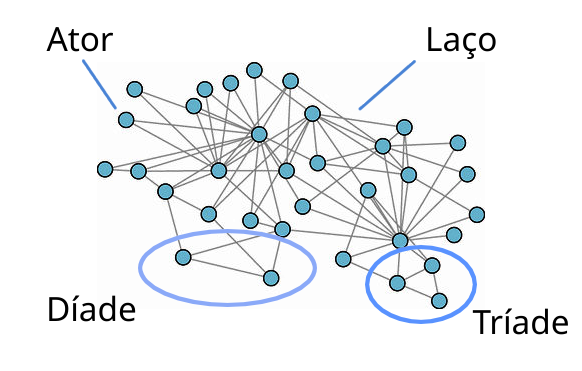
\includegraphics[width=8cm]{imagens/social_network.png}
    \caption{Representação de conceitos de redes sociais.}
    \label{fig:networkDefs}
    \Fonte{O autor.}
\end{figure}

Uma das características mais importantes de uma rede social é o padrão estrutural formado pela organização de seus laços. \citeonline{Christakis2007} indicam que o mesmo conjunto de indivíduos pode apresentar grande variabilidade no modo como completa uma tarefa de acordo com a forma com que seus laços estão organizados; desta maneira, uma rede social cuidadosamente estruturada pode ser tão eficaz quanto uma segunda rede com muito mais atores porém organizada aleatoriamente. Por exemplo, um exército organizado em pequenos esquadrões fortemente conectados apresenta uma efetividade muito superior a um arranjo em fila, onde cada soldado conhece apenas quem está atrás ou em sua frente.

A Figura \ref{fig:structures} apresenta três exemplos de organizações de redes sociais. A primeira, mais à esquerda, consiste em uma estrutura que se assemelha a uma longa fila com laços homogêneos, onde cada ator está ligado com exatamente outros dois atores, exceto pelo primeiro e pelo último; a segunda, no meio, apresenta uma estrutura hierárquica, onde um ator central possui laços dirigidos para outros dois atores, que por sua vez também estão ligados de forma dirigida com outros dois atores distintos, e assim sucessivamente; por fim, a terceira, à direita, apresenta uma rede social contendo dez subconjuntos de atores, cada um contendo dez atores completamente conectados por laços mútuos.

\begin{figure}[ht]
    \centering
    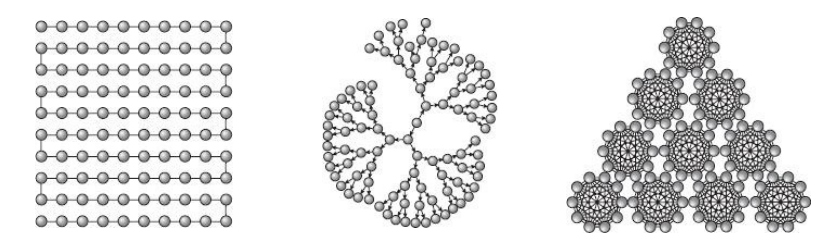
\includegraphics[width=15cm]{imagens/social_structures.png}
    \caption{Três exemplos de estruturas de redes sociais.}
    \label{fig:structures}
    \Fonte{\citeonline{Christakis2007}}
\end{figure}

Tais organizações manifestam-se com alguma frequência em situações sociais reais. Por exemplo, a estrutura hierárquica captura aspectos cruciais de estratégias de marketing multinível ou esquemas de pirâmide, onde há um ator central que detém controle sobre a disseminação de informações pela rede, enquanto a estrutura de subgrupos coesos pode representar uma estratégia de organização militar ou equipes de diferentes setores de uma empresa \cite{Christakis2007}.

Entretanto, no sentido geral, redes sociais tendem a evoluir de forma orgânica, e portanto não apresentam uma homogeneidade tão acentuada como nos exemplos citados. Alguns estudos buscaram investigar como esta evolução ocorre; um dos principais fenômenos identificados foi a \emph{homofilia}\footnote{tradução livre de \textit{homophily}}, que prescreve que indivíduos tendem a formar laços com outros que apresentam características similares \cite{McPherson2001}. Além disso, particularidades de cada indivíduo podem afetar de forma significativa a maneira como laços são formados: por exemplo, indivíduos de natureza introvertida podem tender a possuir círculos sociais menores, enquanto aqueles mais propícios a buscar novas experiências podem exibir uma quantidade de laços acima da média \textit{(ibidem)}.

A Figura \ref{fig:karate}, que exibe a rede de amizades em um clube de karatê de 34 membros, demonstra alguns destes aspectos: dois indivíduos, de identificadores 1 e 34, possuem um grande número de laços imediatos, enquanto outros -- como os atores 16, 15 e 23 -- possuem apenas dois laços imediatos.

\begin{figure}[ht]
    \centering
    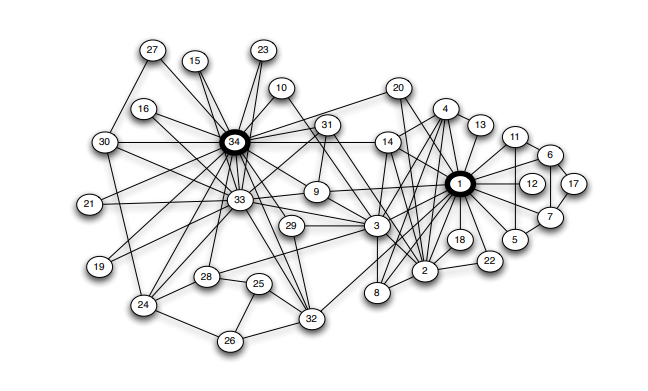
\includegraphics[width=15cm]{imagens/karate.png}
    \caption{Rede social de um clube de karatê}
    \label{fig:karate}
    \Fonte{\citeonline{Easley2010}}
\end{figure}

Apesar desta variabilidade, alguns estudos foram capazes de identificar alguns padrões na distribuição de laços em redes sociais. Um dos mais significativos foi o experimento conduzido por \citeonline{Milgram1967}, onde os participantes recebiam uma carta destinada a uma pessoa desconhecida e deveriam entregá-la a algum indivíduo próximo, que por sua vez deveria repassá-la da mesma forma até que a carta chegasse a seu destinatário. Analisando o percurso das cartas que não foram perdidas, o autor observou que a maioria delas necessitou de aproximadamente seis repasses, descrevendo assim o Fenômeno do Mundo Pequeno e cunhando a expressão "seis graus de separação".

Ao longo do restante desta seção, dará-se maior ênfase na descrição dos processos de disseminação de influência através de redes sociais, assim como algumas características de grupos sociais no contexto educacional.

\subsection{Influência Social e seus Efeitos} \label{sec:socialinfluence}

Segundo \citeonline{Simons-Morton2010}, a influência social representa o efeito que outros causam sobre os comportamentos e atitudes de indivíduos ou grupos. A influência pode originar-se tanto de pessoas muito próximas, com as quais o invidíduo em questão possui um relacionamento íntimo, quanto de pessoas mais distantes, com as quais existe um laço social direto porém o mesmo não é muito intenso \cite{Berkman2000}. Entretanto, até mesmo pessoas desconhecidas podem causar algum nível de influência; uma demonstração deste fenômeno foi relatada na pesquisa de \citeonline{Fowler2008}, que identificou que a disseminação de felicidade em uma rede estudada durante 20 anos se estende por até três graus de separação (ou seja, pode advir de amigos de amigos de amigos). Na figura \ref{fig:socialzones}, tem-se uma representação das zonas de contato social entre indivíduos.

\begin{figure}[ht]
    \centering
    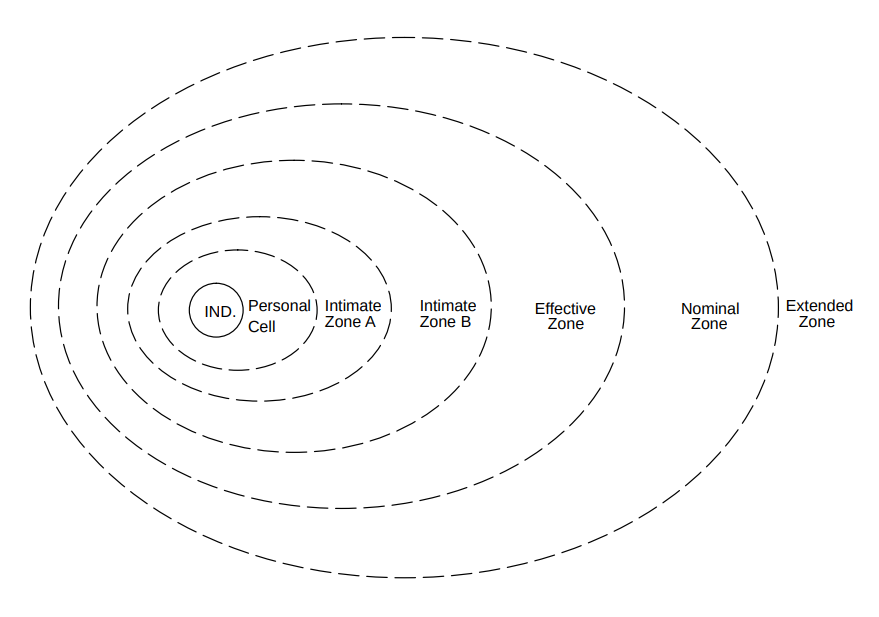
\includegraphics[width=12cm]{imagens/zones.png}
    \caption{Zonas de contato social.}
    \label{fig:socialzones}
    \Fonte{\citeonline{Berkman2000}}
\end{figure}

O modelo apresentado pela figura foi descrito por \citeonline{Berkman2000} com base em outros estudos sobre influência social e níveis de contato. Neste modelo, tem-se seis zonas sociais: (i) \textit{personal cell} (célula pessoal), que representa os familiares mais próximos e os mais íntimos dos amigos; (ii) \textit{intimate zone A} (zona íntima A), que representa familiares próximos e amizades íntimas ativas; (iii) \textit{intimate zone B} (zona íntima B), que consiste em familiares e amigos emocionalmente importantes mas com um cunho mais passivo; (iv) \textit{effective zone} (zona efetiva), composta por pessoas com as quais o relacionamento é mantido devido a razões de necessidade cotidiana; (v) \textit{nominal zone} (zona nominal), que contém apenas pessoas que o indivíduo conhece mas que não apresentam grande importância; e (vi) \textit{extended zone} (zona estendida), que consiste em pessoas distantes com as quais não há quase nenhum contato, porém o indivíduo em questão as conhece pelo menos de rosto.

\citeonline{Berkman2000} argumenta que todas as zonas do modelo apresentam importância considerável, não somente os círculos mais internos. Apesar de estes serem extremamente importantes para a manutenção da saúde emocional, indivíduos que pertencem à zona efetiva, nominal ou estendida fornecem suporte instrumental -- ou seja, auxiliam na execução de alguma tarefa ou na conquista de algum objetivo. Assim, tais indivíduos podem causar mudanças de comportamento e portanto também são agentes de influência social, mesmo que de forma menos acentuada.

Tratando das consequências da influência social, \citeonline{Steinberg2007} relatam que, assim como outros estudos conduzidos previamente evidenciaram, a adoção de hábitos perigosos e nocivos -- como abuso de substâncias, delinquência e imprudência no trânsito -- aumenta significativamente no período da adolescência, primariamente devido à maior susceptibilidade a pressão de pares, e estabiliza à medida que o indivíduo atinge a idade adulta.

Entretanto, este padrão também se mantém para condutas neutras ou até mesmo socialmente valorizadas, como tirar notas boas ou evitar drogas. Os autores sugerem que tal comportamento pode ser causado pela noção de que os pares de um indivíduo representam um ponto de referência comportamental que deve ser seguido, caracterizando o grupo social como um ambiente que tende à homogeneidade -- em caso de visões conflitantes, o indivíduo que foge à regra pode sofrer uma série de efeitos negativos, como rejeição, ostracismo e exclusão do grupo \cite{Steinberg2007,Gremmen2017}.

\subsection{Redes Sociais no Contexto Educacional} \label{sec:networkseducation}

A influência social e a disseminação de comportamento também causam profundos efeitos sobre os hábitos de estudantes, especialmente devido à grande quantidade de tempo que estes passam interagindo com seus colegas de classe, sendo esta uma característica observada principalmente no período da adolescência \cite{Butler-Barnes2015}. Na literatura científica, tem-se um considerável arcabouço de estudos que investigam padrões de características de propagação de influência e de que forma seus efeitos se manifestam nos estudantes, buscando correlações entre seu contexto social e outras variáveis de interesse \cite{Flashman2012,Gremmen2017,Farmer1996,Blansky2013,Rambaran2017,Berndt1990}.

\citeonline{Goodenow1993} argumentam que a motivação acadêmica não pode ser analisada como um fenômeno exclusivamente individual, pois este é afetado profundamente pelas relações sociais e laços de amizade dos estudantes. As autoras também sugerem que a sensação de pertencimento à escola e a influência dos valores de amigos são fatores altamente importantes quando se trata de motivação acadêmica, sendo que este último apresenta um nível de correlação levemente inferior -- porém, no quesito da valorização das atividades acadêmicas, a influência das amizades apresentou correlação elevada. O estudo também identificou que o impacto do pertencimento é mais significativo em grupos com maior risco de evasão escolar.

Reforçando a noção do impacto do contexto social de estudantes sobre seu comportamento escolar, \citeonline{Rice2013} identificaram que alunos relatam atitudes e percepções mais positivas, além de maior autoconfiança, acerca do estudo de matemática e ciências quando estes recebem suporte social abundante de seus seus pais, professores e amigos. O trabalho identificou que todos os três fatores apresentam correlações similares entre si (sendo todas positivas e estatisticamente significantes), porém o relato dos alunos amostrados sugere que o suporte social do grupo de amigos é consideravelmente inferior ao suporte oferecido por pais e professores. Sendo assim, sugere-se que a influência de laços de amizade merece um estudo mais aprofundado, por ser um fator destoante dos demais.
%% DEPRECATED !!!

% \subsection{Influência Social e seus Efeitos} \label{sec:socialinfluence}

% Segundo \citeonline{Simons-Morton2010}, a influência social representa o efeito que outros causam sobre os comportamentos e atitudes de indivíduos ou grupos. A influência pode originar-se tanto de pessoas muito próximas, com as quais o invidíduo em questão possui um relacionamento íntimo, quanto de pessoas mais distantes, com as quais existe um laço social direto porém o mesmo não é muito intenso \cite{Berkman2000}. Entretanto, até mesmo pessoas desconhecidas podem causar algum nível de influência; uma demonstração deste fenômeno foi relatada na pesquisa de \citeonline{Fowler2008}, que identificou que a disseminação de felicidade em uma rede estudada durante 20 anos se estende por até três graus de separação (ou seja, pode advir de amigos de amigos de amigos). Na figura \ref{fig:socialzones}, tem-se uma representação das zonas de contato social entre indivíduos.

% \begin{figure}
%     \centering
%     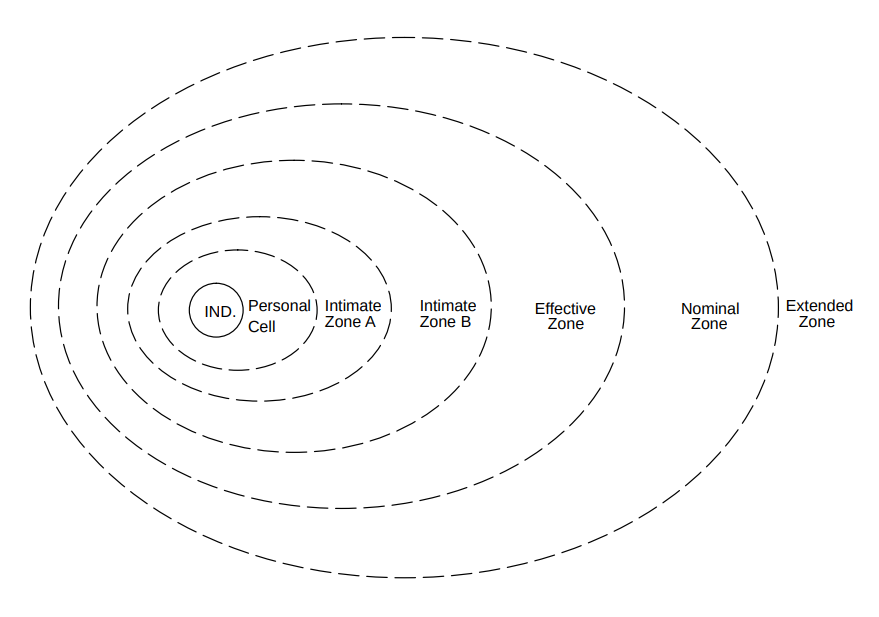
\includegraphics[width=12cm]{imagens/zones.png}
%     \caption{Zonas de contato social. Fonte: \cite{Berkman2000}}
%     \label{fig:socialzones}
% \end{figure}

% O modelo apresentado pela figura foi descrito por \citeonline{Berkman2000} com base em outros estudos sobre influência social e níveis de contato. Neste modelo, tem-se seis zonas sociais: (i) \textit{personal cell} (célula pessoal), que representa os familiares mais próximos e os mais íntimos dos amigos; (ii) \textit{intimate zone A} (zona íntima A), que representa familiares próximos e amizades íntimas ativas; (iii) \textit{intimate zone B} (zona íntima B), que consiste em familiares e amigos emocionalmente importantes mas com um cunho mais passivo; (iv) \textit{effective zone} (zona efetiva), composta por pessoas com as quais o relacionamento é mantido devido a razões de necessidade cotidiana; (v) \textit{nominal zone} (zona nominal), que contém apenas pessoas que o indivíduo conhece mas que não apresentam grande importância; e (vi) \textit{extended zone} (zona estendida), que consiste em pessoas distantes com as quais não há quase nenhum contato, porém o indivíduo em questão as conhece pelo menos de rosto.

% \citeonline{Berkman2000} argumenta que todas as zonas do modelo apresentam importância considerável, não somente os círculos mais internos. Apesar de estes serem extremamente importantes para a manutenção da saúde emocional, indivíduos que pertencem à zona efetiva, nominal ou estendida fornecem suporte instrumental -- ou seja, auxiliam na execução de alguma tarefa ou na conquista de algum objetivo. Assim, tais indivíduos podem causar mudanças de comportamento e portanto também são agentes de influência social, mesmo que de forma menos acentuada.

% Tratando das consequências da influência social, \citeonline{Steinberg2007} relatam que, assim como outros estudos conduzidos previamente evidenciaram, a adoção de hábitos perigosos e nocivos -- como abuso de substâncias, delinquência e imprudência no trânsito -- aumenta significativamente no período da adolescência, primariamente devido à maior susceptibilidade a pressão de pares, e estabiliza à medida que o indivíduo atinge a idade adulta.

% Entretanto, este padrão também se mantém para condutas neutras ou até mesmo socialmente valorizadas, como tirar notas boas ou evitar drogas. Os autores sugerem que tal comportamento pode ser causado pela noção de que os pares de um indivíduo representam um ponto de referência comportamental que deve ser seguido, caracterizando o grupo social como um ambiente que tende à homogeneidade -- em caso de visões conflitantes, o indivíduo que foge à regra pode sofrer uma série de efeitos negativos, como rejeição, ostracismo e exclusão do grupo \cite{Steinberg2007}.

% \subsection{Redes Sociais no Contexto Educacional} \label{sec:networkseducation}

% A influência social e a disseminação de comportamento também causam profundos efeitos sobre os hábitos de estudantes, especialmente devido à grande quantidade de tempo que estes passam interagindo com seus colegas de classe, sendo esta uma característica observada principalmente no período da adolescência \cite{Butler-Barnes2015}. Na literatura científica, tem-se um considerável arcabouço de estudos que investigam padrões de características de propagação de influência e de que forma seus efeitos se manifestam nos estudantes, buscando correlações entre seu contexto social e outras variáveis de interesse \cite{Flashman2012,Gremmen2017,Farmer1996,Blansky2013,Rambaran2017,Berndt1990}.

% \citeonline{Goodenow1993} argumentam que a motivação acadêmica não pode ser analisada como um fenômeno exclusivamente individual, pois este é afetado profundamente pelas relações sociais e laços de amizade dos estudantes. As autoras também sugerem que a sensação de pertencimento à escola e a influência dos valores de amigos são fatores altamente importantes quando se trata de motivação acadêmica, sendo que este último apresenta um nível de correlação levemente inferior -- porém, no quesito da valorização das atividades acadêmicas, a influência das amizades apresentou correlação elevada. O estudo também identificou que o impacto do pertencimento é mais significativo em grupos com maior risco de evasão escolar.

% Reforçando a noção do impacto do contexto social de estudantes sobre seu comportamento escolar, \citeonline{Rice2013} identificaram que alunos relatam atitudes e percepções mais positivas, além de maior autoconfiança, acerca do estudo de matemática e ciências quando estes recebem suporte social abundante de seus seus pais, professores e amigos. O trabalho identificou que todos os três fatores apresentam correlações similares entre si (sendo todas positivas e estatisticamente significantes), porém o relato dos alunos amostrados sugere que o suporte social do grupo de amigos é consideravelmente inferior ao suporte oferecido por pais e professores. Sendo assim, sugere-se que a influência de laços de amizade merece um estudo mais aprofundado, por ser um fator destoante dos demais.
%% DEPRECATED!!!!

% \subsection{Redes Sociais no Contexto Educacional} \label{sec:networkseducation}

% A influência social e a disseminação de comportamento também causam profundos efeitos sobre os hábitos de estudantes, especialmente devido à grande quantidade de tempo que estes passam interagindo com seus colegas de classe, sendo esta uma característica observada principalmente no período da adolescência \cite{Butler-Barnes2015}. Na literatura científica, tem-se um considerável arcabouço de estudos que investigam padrões de características de propagação de influência e de que forma seus efeitos se manifestam nos estudantes, buscando correlações entre seu contexto social e outras variáveis de interesse \cite{Flashman2012,Gremmen2017,Farmer1996,Blansky2013,Rambaran2017,Berndt1990}.

% \citeonline{Goodenow1993} argumentam que a motivação acadêmica não pode ser analisada como um fenômeno exclusivamente individual, pois este é afetado profundamente pelas relações sociais e laços de amizade dos estudantes. As autoras também sugerem que a sensação de pertencimento à escola e a influência dos valores de amigos são fatores altamente importantes quando se trata de motivação acadêmica, sendo que este último apresenta um nível de correlação levemente inferior -- porém, no quesito da valorização das atividades acadêmicas, a influência das amizades apresentou correlação elevada. O estudo também identificou que o impacto do pertencimento é mais significativo em grupos com maior risco de evasão escolar.

% Reforçando a noção do impacto do contexto social de estudantes sobre seu comportamento escolar, \citeonline{Rice2013} identificaram que alunos relatam atitudes e percepções mais positivas, além de maior autoconfiança, acerca do estudo de matemática e ciências quando estes recebem suporte social abundante de seus seus pais, professores e amigos. O trabalho identificou que todos os três fatores apresentam correlações similares entre si (sendo todas positivas e estatisticamente significantes), porém o relato dos alunos amostrados sugere que o suporte social do grupo de amigos é consideravelmente inferior ao suporte oferecido por pais e professores. Sendo assim, sugere-se que a influência de laços de amizade merece um estudo mais aprofundado, por ser um fator destoante dos demais.
\section{Teoria dos Grafos e Redes Complexas} \label{sec:graphtheory}

Grafos são constructos matemáticos compostos por pontos, denominados vértices ou nós, que podem estar conectados por linhas, denominadas arestas ou arcos, dependendo da presença ou ausência de direção nas mesmas \cite{Bondy1976}. Tais objetos podem ser empregados na representação de uma grande variedade de situações e problemas reais, como cadeias alimentares ou redes tróficas, o conjunto de vasos sanguíneos de um corpo, redes metabólicas, complexos de proteínas, redes neurais biológicas, redes de colaboração entre pesquisadores, relações de negócio entre corporações, redes ferroviárias e a própria Internet, além de outros exemplos \cite{Newman2003}.

Naturalmente, grafos também podem ser utilizados para representar redes sociais, exploradas na Seção \ref{sec:socialnetworks}, de forma muito conveniente: os vértices do grafo representam atores, enquanto as arestas ou arcos simbolizam os laços entre os mesmos \cite{Newman2003}. Desta maneira, é possível apropriar-se de grande parte da literatura da Teoria dos Grafos no desenvolvimento de estudos sobre redes sociais, favorecendo uma compreensão mais concreta de seus conceitos matemáticos abstratos.

A definição de grafos é essencialmente genérica, isto é, não há nenhuma suposição quanto a existência ou não de padrões formados por suas arestas ou quanto à qualquer característica de seus vértices. Adicionalmente, não há nenhuma delimitação quanto ao número de vértices ou arestas presentes no grafo; por consequência, um grafo pode possuir 10 vértices e nenhuma aresta, ou um vértice e 10 arcos ligando-o a si próprio (um tipo de arco conhecido na literatura como laço reflexivo\footnote{tradução livre de \textit{self-loop}}), ou até mesmo uma quantidade infinita de vértices e arestas, formando um grafo infinito \cite{Bondy1976}.

Entretanto, dada a ubiquidade da modelagem de sistemas e situações reais como grafos, definiu-se o termo \emph{Rede Complexa} para denominar grafos cujas topologias apresentam características similares a redes observáveis no mundo real, onde ordem e desordem coexistem \cite{Fortunato2010}. Sendo assim, um grafo aleatório formado a partir do modelo de \citeonline{Erdos1959} não pode ser considerado uma rede complexa, por apresentar alto índice de homogeneidade na distribuição de suas arestas, enquanto a rede social do clube de karatê, apresentada na Figura \ref{fig:karate}, pode ser considerada um exemplo típico de rede complexa.

O presente trabalho aborda exclusivamente redes sociais, e portanto fará uso principalmente da literatura científica acerca de redes complexas, visto que a grande maioria das redes sociais são instâncias de redes complexas. Consequentemente, verifica-se a necessidade de esclarecer a seguinte hierarquia de nomenclaturas, em ordem de especificidade crescente:

\begin{alineas}
    \item Grafo: empregado ao tratar de assuntos que se aplicam a qualquer arranjo de vértices e arestas, especialmente em contextos matemáticos;
    \item Rede complexa: termo utilizado na discussão de grafos com topologia não-trivial, com características observáveis comumente no mundo real;
    \item Rede social: especialização de rede complexa, onde vértices representam atores (indivíduos) e arestas representam laços (relacionamento interpessoal de qualquer natureza).
\end{alineas}

A Figura \ref{fig:networknomenclature} apresenta uma demonstração gráfica da distinção entre estes três termos, onde: o grafo (a) consiste em um arranjo puramente arbitrário com propriedades matemáticas particulares \cite{Bondy1976}; a rede complexa (b) consiste em um conjunto de páginas da \textit{web} com arcos representando os \textit{hyperlinks} entre as páginas \cite{Fortunato2010}; e a rede social (c) consiste em uma rede de co-autoria de artigos científicos na área de detecção de comunidades em redes complexas \cite{Newman2004}.

\begin{figure}[ht]
    \centering
    \begin{subfigure}{0.36\textwidth}
        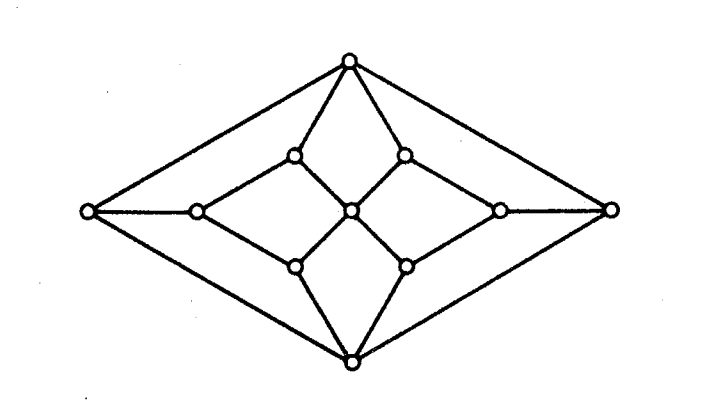
\includegraphics[width=\linewidth]{imagens/generic_graph.png}
        \caption{Grafo} \label{fig:1a}
    \end{subfigure}
    \vspace*{0.2cm}
    %\hspace*{\fill} % separation between the subfigures
    \begin{subfigure}{0.31\textwidth}
        \includegraphics[width=\linewidth]{imagens/complex_network2.png}
        \caption{Rede Complexa} \label{fig:1b}
    \end{subfigure}
    \\
    %\hspace*{\fill} % separation between the subfigures
    \begin{subfigure}{0.54\textwidth}
        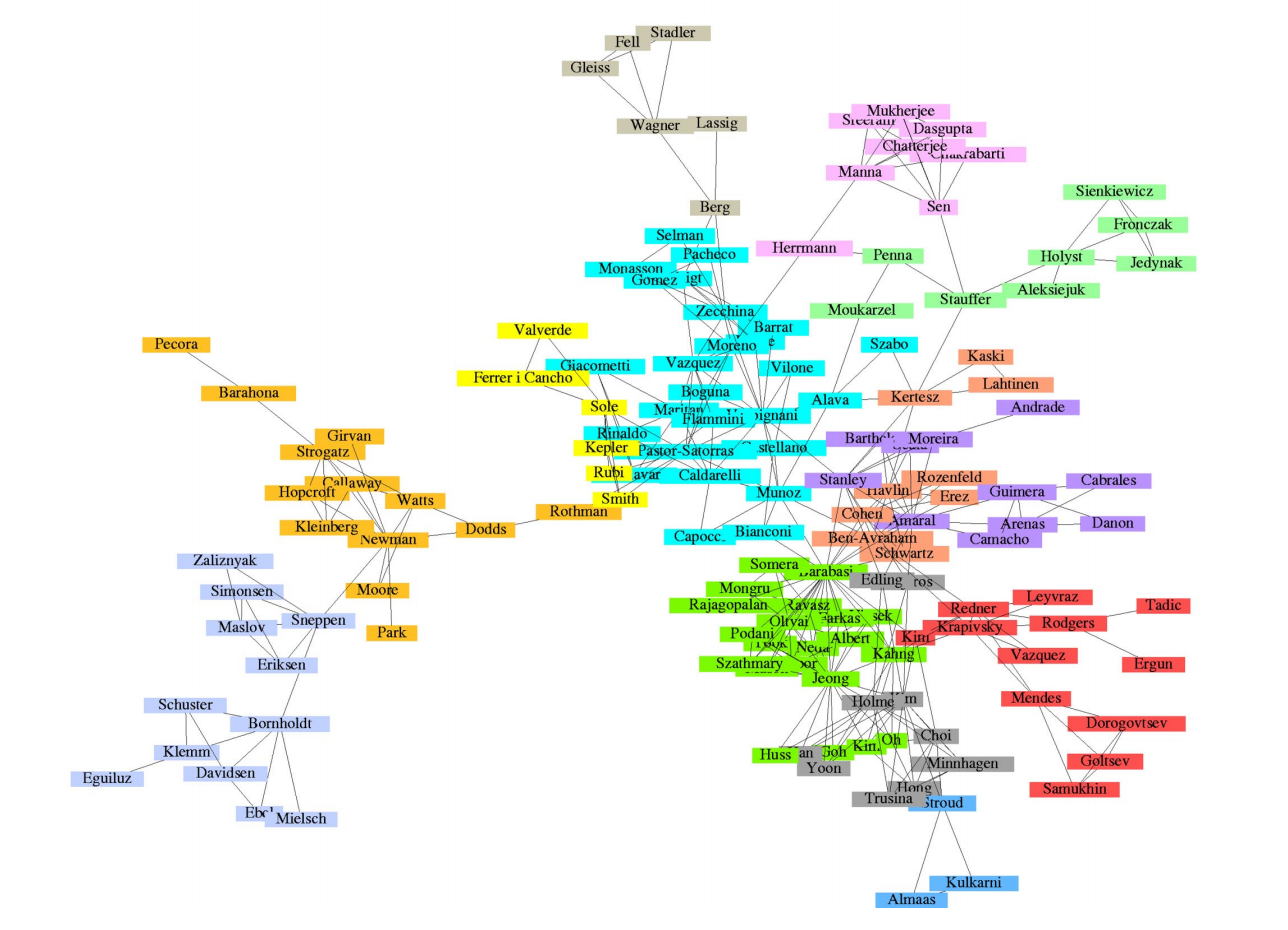
\includegraphics[width=\linewidth]{imagens/collaboration_network.png}
        \caption{Rede Social} \label{fig:1c}
    \end{subfigure}
    \vspace*{0.3cm}
    \caption{Distinção entre nomenclaturas}
    \label{fig:networknomenclature}
    \Fonte{Adaptado de \citeonline{Bondy1976}, \citeonline{Fortunato2010} e \citeonline{Newman2004}.}
\end{figure}

\subsection{Conceitos Fundamentais} \label{sec:graphfoundation}

Segundo \citeonline{Harary1969}, a terminologia e notação matemática empregadas na descrição de grafos varia frequentemente de trabalho para trabalho; portanto, é sugerido que cada autor esclareça com antecedência de que forma um grafo será descrito. Neste estudo, grafos serão tratados como pares $G = (V, E)$, onde $V$ consiste no conjunto de vértices, e o conjunto $E$ representa as arestas do grafo, composto por pares de nós $\{u, v\}$.

Caso as arestas do grafo possuam direção -- ou seja, se a aresta entre $u$ e $v$ for independente da aresta entre $v$ e $u$ --, terá-se um grafo dirigido, onde o termo ``arestas'' e seu conjunto $E$ é substituído por ``arcos'', os quais são representados por um conjunto $A$ de pares ordenados $(u, v)$. Em grafos dirigidos, um arco de $u$ até $v$ pode ser completamente diferente do arco na direção oposta, de $v$ até $u$; além disso, um deles pode existir sem o outro. O termo ``ligação'' será utilizado para referir-se a arcos e arestas de forma indistinta, assim como o termo ``laço'' (equivalente) foi utilizado na Seção \ref{sec:socialnetworks}.

Ao longo de toda a extensão deste trabalho, todos os grafos estudados serão simples; isto é, entre quaisquer vértices $u$ e $v$, pode existir somente uma ou nenhuma aresta $\{u, v\}$ ou, caso o grafo seja dirigido, pode existir nenhum arco, um arco $(u, v)$, um arco $(v, u)$, ou ambos os arcos. Além disso, não são permitidos \textit{loops} ou laços reflexivos, onde uma ligação possui origem igual ao seu destino. Grafos que permitem \textit{loops} e múltiplas ligações entre dois vértices são denominados multigrafos \cite{Newman2010}.

Além de simplesmente existirem ou não, ligações podem possuir um valor associado, denominado peso. Este valor pode representar uma grande variedade de conceitos, como distância entre cidades, a largura de banda entre dois pontos de rede, a impedância ou corrente entre duas extremidades em um circuito elétrico ou a frequência de contato ou amizade entre dois indivíduos (atores) \cite{Newman2010}. Caso as ligações possuam peso, o grafo é denominado ponderado.

A literatura da Teoria dos Grafos define diversos outros termos, com diferentes níveis de especificidade. Alguns destes, selecionados por apresentarem maior relevância neste estudo, são definidos da seguinte forma:

\begin{alineas}
    \item Grau: para um vértice $u$, seu grau é definido como a quantidade de vértices ligados a $u$ por uma aresta. Em grafos dirigidos, o grau se divide em grau de entrada (arcos com destino em $u$) e grau de saída (arcos com origem em $u$);
    \item Subgrafo: um grafo $G'$ derivado de $G$ cujo conjunto de vértices $V'$ consiste em um subconjunto de $V$. As ligações de $G'$ podem existir somente entre os vértices de $V'$;
    \item Grafo completo: um grafo onde, para todos os vértices $u$ e $v$, existe uma aresta $\{u, v\}$ ou, caso o grafo seja dirigido, ambos os arcos $(u, v)$ e $(v, u)$ estão presentes. Em outras palavras, todos os vértices estão ligados a todos os outros. Grafos completos são tipicamente denominados $K_n$, com $n = |V|$ (número de vértices);
    \item Clique: um subgrafo de $G$ que, tomado de forma isolada, consiste em um grafo completo; % talvez não precise
    \item Caminho: uma sequência de vértices com origem em $u$ e destino em $v$ tal que cada vértice da sequência está conectado ao próximo por uma ligação. A distância do caminho é igual ao somatório dos pesos das ligações\footnote{caso o grafo seja não-ponderado, considera-se que o peso da ligação é igual a 1.}. Caso não exista nenhum outro caminho entre $u$ e $v$ com distância menor, tem-se um caminho denominado \emph{caminho mínimo};
    \item Matriz de adjacências: representação matemática de um grafo, que consiste em uma matriz quadrada de ordem dada por $|V|$. Cada célula indica se existe ou não uma aresta ou arco entre os vértices representados pela combinação de linha (origem) e coluna (destino). Caso não haja ligação, a célula terá valor 0; caso contrário, o valor será o peso da ligação ou 1. Em grafos simples, a diagonal principal é sempre composta por zeros.
\end{alineas}

\subsection{Centralidade} \label{sec:centrality}

Segundo \cite{Newman2010}, há um volume expressivo de estudos referentes ao conceito de centralidade em redes complexas. Em linhas gerais, a medida de centralidade busca identificar quais são os vértices mais importantes em uma rede complexa; no entanto, a própria definição de ``importante'' é subjetiva e aberta a questionamentos, e consequentemente diversas métricas de centralidade foram desenvolvidas ao longo das décadas recentes.

Historicamente, a centralidade tem sido estudada principalmente no contexto de redes sociais \cite{Bavelas1948,Newman2010}; no entanto, aplicações em outras áreas também vem sendo publicadas, como em rotas de comércio no planejamento urbano \cite{Pitts1965}, redes de citação e colaboração científica \cite{Newman2001} e disseminação de epidemias \cite{Santiago2019}. % Revisar a citação e colaboração científica (é social em teoria)

O Quadro \ref{board:centralities} enumera algumas das principais métricas de centralidade, identificando seus conceitos ou ideias gerais de forma breve de acordo com autores da área \cite{Newman2010,Grando2015}.


\begin{quadro}[ht]
    \caption{Sumário de métricas de centralidade}
    \label{board:centralities}
    \fontsize{10}{12}\selectfont
    \def\arraystretch{1.25}
    \begin{tabularx}{\textwidth}{|c|c|Y|}
        \hline
        \textbf{Métrica} & \textbf{Tradução livre} & \textbf{Conceito}
        \\ \hline
        \textit{Degree Centrality} & Grau & Visibilidade, atividade de comunicação
        \\ \hline
        \textit{Betweenness Centrality} & Intermediação & Controle de comunicação, ação como ponte
        \\ \hline
        \textit{Closeness Centrality} & Proximidade & Independência, eficiência
        \\ \hline
        \textit{Eigenvector Centrality} & Autovalor & Importância proporcional à importância dos contatos
        \\ \hline
        \textit{Katz Centrality} & -- & Variante de Autovalor com um parâmetro constante. Mais apropriada para grafos dirigidos
        \\ \hline
    \end{tabularx}
\end{quadro}

Visando habilitar uma compreensão mais ampla sobre as cinco métricas de centralidade descritas, a Figura \ref{fig:centralities} apresenta visualmente cada uma delas aplicadas sobre uma rede complexa arbitrária. Cores azuis representam centralidade baixa, enquanto cores tendendo ao vermelho escuro indicam centralidade alta.

\begin{figure}[ht]
    \centering
    \vspace*{0.4cm}
    \begin{subfigure}{0.27\textwidth}
        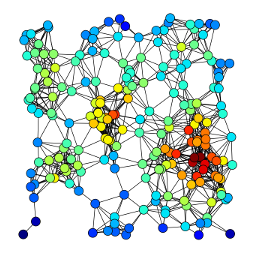
\includegraphics[width=\linewidth]{imagens/degree.png}
        \caption{Grau} \label{fig:degree}
    \end{subfigure}
    \begin{subfigure}{0.27\textwidth}
        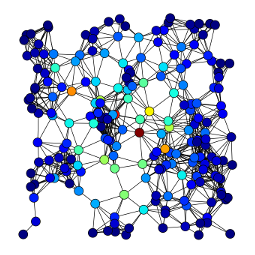
\includegraphics[width=\linewidth]{imagens/betweenness.png}
        \caption{Intermediação} \label{fig:betweenness}
    \end{subfigure}
    \begin{subfigure}{0.27\textwidth}
        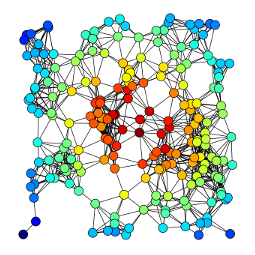
\includegraphics[width=\linewidth]{imagens/closeness.png}
        \caption{Proximidade} \label{fig:closeness}
    \end{subfigure}
    \\
    \vspace*{0.2cm}
    %\hspace*{\fill} % separation between the subfigures
    \begin{subfigure}{0.27\textwidth}
        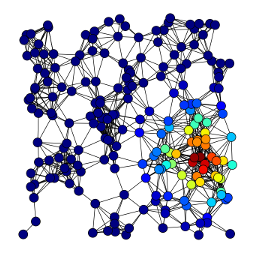
\includegraphics[width=\linewidth]{imagens/eigenvector.png}
        \caption{Autovalor} \label{fig:eigenvector}
    \end{subfigure}
    \begin{subfigure}{0.27\textwidth}
        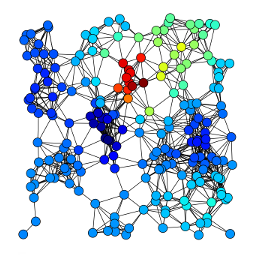
\includegraphics[width=\linewidth]{imagens/katz.png}
        \caption{Katz} \label{fig:katz}
    \end{subfigure}
    
    \vspace*{0.3cm}
    \RaggedRight
    \caption{Visualização de métricas de centralidade.}
    \label{fig:centralities}
    \Fonte{Wikimedia Commons}
\end{figure}

\subsubsection{Grau} \label{sec:degree}

O grau de um vértice, definido na Seção \ref{sec:graphfoundation} caracteriza uma medida bastante rudimentar e simplória de sua centralidade ou importância. Apesar disso, existem argumentos a favor de seu uso, pois a métrica fornece uma percepção razoável acerca da visibilidade do vértice no grafo \cite{Newman2010}.

Além disso, indivíduos com muitas ligações em uma rede social podem possuir maior influência ou mais facilidade no acesso à informação, enquanto artigos citados por muitos outros em uma rede científica podem ser mais impactantes ou influentes em sua área de pesquisa (ibidem).

Em grafos dirigidos, a centralidade por grau se desdobra em grau de entrada e grau de saída, sendo que ambas são, em geral, igualmente importantes \cite{Newman2010}. A centralidade por grau de entrada de um vértice $v_k$ qualquer pode ser definida da seguinte forma:

\begin{equation}
    \label{eq:indegree}
    C_{G_{entrada}}(v_k) = \sum_{i=1}^{|V|} w(v_i, v_k)
\end{equation}

\noindent enquanto sua centralidade por grau de saída é definida da seguinte maneira:

\begin{equation}
    \label{eq:outdegree}
    C_{G_{saida}}(v_k) = \sum_{i=1}^{|V|} w(v_k, v_i)
\end{equation}

\noindent onde $C_G$ representa o nível de centralidade por grau de entrada ou saída, $|V|$ representa o número de vértices do grafo e $w(v_i, v_j)$ representa o peso da ligação com origem em $v_i$ e destino em $v_j$, onde o peso é considerado 1 se o grafo não for ponderado e 0 se a ligação não existe.

\subsubsection{Intermediação} \label{sec:betweenness}

A intermediação (do inglês \textit{betweenness}) foi proposta por \citeonline{Freeman1977} como uma métrica de centralidade que busca medir o nível com que um vértice se põe no caminho de outros vértices. Para calculá-la, computa-se inicialmente os caminhos mínimos de todos os vértices do grafo para todos os outros (ou seja, $|V|^2$ caminhos). Posteriormente, verifica-se de quantos destes caminhos o vértice sendo medido faz parte; quanto maior este número, maior será sua centralidade por intermediação.

\citeonline{Newman2010} sugere que a importância de vértices com elevada centralidade por intermediação deriva da sua capacidade de controlar a informação que trafega pelo grafo, visto que os caminhos mínimos são geralmente mais usados do que os demais em diversos contextos. Por exemplo, em uma rede de computadores, um nó com alto nível de intermediação tipicamente é responsável por encaminhar um grande volume de pacotes. Neste sentido, se o mesmo for comprometido por um agente malicioso, a segurança de grande parte da rede pode ser violada; adicionalmente, se o mesmo for removido da rede, poderá ocorrer uma disrupção significativa na comunicação entre os nós.

A intermediação se difere de boa parte das outras métricas de centralidade por não medir quão bem conectado um vértice está, mas sim até que ponto o mesmo age como uma ``ponte'' entre outros vértices. Portanto, um vértice com pouquíssimas ligações imediatas pode possuir uma alta centralidade por intermediação \cite{Newman2010}. Matematicamente, a intermediação de um vértice $v_k$ qualquer pode ser definida como:

\begin{equation}
    \label{eq:betweenness}
    C_I(v_k) = \sum_{i=1}^{|V|} \sum_{j=1}^{|V|} \frac{g_{v_k}(v_i, v_j)}{g(v_i, v_j)}
\end{equation}

\noindent onde $C_I$ representa a centralidade por intermediação, $g_{v_k}(v_i, v_j)$ indica o número de caminhos mínimos com origem em $v_i$ e destino em $v_j$ que passam por $v_k$ e $g(v_i, v_j)$ simboliza o número total de caminhos mínimos entre $v_i$ e $v_j$. A Figura \ref{fig:star} apresenta um exemplo de grafo com topologia de estrela, onde o vértice central apresenta intermediação máxima: todos os vértices precisam passar por ele para atingir outro.

\begin{figure}[ht]
    \centering
    
\includegraphics[width=7cm]{imagens/star.png}
    \caption{Um grafo de estrela, onde um vértice intermedia todas as interações.}
    \label{fig:star}
    \Fonte{\citeonline{Newman2010}}
\end{figure}

A centralidade por intermediação pode ser aplicada sem alterações em grafos dirigidos, visto que os arcos que ligam os vértices de um caminho devem ter origem no atual e destino no próximo da sequência. Além disso, a intermediação pode também ser aplicada em grafos ponderados, pois a definição de um caminho mínimo já leva em consideração o peso das ligações, conforme descrito na Seção \ref{sec:graphfoundation}.

\subsubsection{Proximidade} \label{sec:closeness}

A centralidade por proximidade (do inglês \textit{closeness}) caracteriza-se, conforme inicialmente definida por \citeonline{Bavelas1950}, como uma métrica de quão próximo o vértice em questão se encontra dos demais, sendo que a proximidade pode ser compreendida como o inverso da distância entre vértices. Concretamente, as distâncias são medidas através do cômputo de todos os caminhos mínimos com origem no vértice sob consideração e destino em cada um dos outros vértices do grafo (ou seja, $|V|$ caminhos).

\citeonline{Newman2010} interpreta a centralidade por proximidade como uma métrica que representa a facilidade de acesso à informação e influência direta sobre outros vértices. Já \citeonline{Grando2015} compreendem que a métrica caracteriza independência, pois vértices próximos dos demais não dependem dos outros para que possam se comunicar, influenciar ou atingir e serem atingidos de qualquer maneira por outros vértices do grafo.

Como seu cálculo depende intimamente de caminhos mínimos, a proximidade também pode ser aplicada em grafos dirigidos e ponderados, assim como a centralidade por intermediação, descrita na Seção \ref{sec:betweenness}. Entretanto, assim como na centralidade por grau, a proximidade também se desdobra em proximidade de entrada e de saída, pois a distância de um caminho de $u$ a $v$ pode ser diferente da distância de $v$ a $u$. Equação \ref{eq:incloseness} indica como a centralidade por proximidade de entrada é calculada para um vértice $v_k$ qualquer, enquanto a Equação \ref{eq:outcloseness} define a centralidade por proximidade de saída.

\begin{equation}
    \label{eq:incloseness}
    C_{P_{entrada}}(v_k) = \frac{|V|}{\sum_{i=1}^{|V|} d(v_i, v_k)}
\end{equation}

\begin{equation}
    \label{eq:outcloseness}
    C_{P_{saida}}(v_k) = \frac{|V|}{\sum_{i=1}^{|V|} d(v_k, v_i)}
\end{equation}

Nestas equações, $C_p$ expressa a centralidade por proximidade de entrada ou saída e $d(v_i, v_j)$ representa a distância do caminho mínimo com origem em $v_i$ e destino em $v_j$. O somatório das distâncias é situado no denominador para efetuar a inversão: quanto maior as distâncias, menor será o valor de centralidade por proximidade, e vice-versa. O numerador $|V|$ é utilizado para normalizar o resultado de acordo com o tamanho do grafo.

\subsubsection{Autovalor} \label{sec:eigenvector}

A centralidade por autovalor foi desenvolvida por \citeonline{Bonacich1987} como uma tentativa de aprimorar a centralidade por grau, definida na Seção \ref{sec:degree}. Segundo o autor, o grau de um vértice captura somente o número de vértices ligados a ele, sem levar em consideração quão importantes os mesmos são. Assim, a centralidade por autovalor caracteriza a importância de um vértice $u$ de forma recursiva -- isto é, conforme mais importantes os vértices ligados a $u$ forem, mais importante $u$ será. Desta maneira, um vértice pode ser importante tanto por estar ligado a um grande número de vértices quanto por estar ligado a poucos vértices cujas importâncias são elevadas.

Em essência, tem-se dois termos adicionais na função de centralidade por grau, que pode ser verificada nas Equações \ref{eq:indegree} e \ref{eq:outdegree}. O primeiro envolve a inclusão de um coeficiente constante ao somatório, habilitando sua normalização e assim tornando a equação mais genérica. O segundo, por sua vez, trata da seguinte modificação: ao invés de considerar somente o peso das ligações, adiciona-se uma multiplicação pela centralidade do vértice oposto, concretizando o conceito desta métrica \cite{Newman2010}. A Equação \ref{eq:eigenvector1} apresenta estas alterações.

\begin{equation}
    \label{eq:eigenvector1}
    C_A(v_k) = \frac{1}{r} \sum_{i=1}^{|V|} w(v_i, v_k) \cdot C_A(v_i) % talvez remover o \cdot
\end{equation}

É possível reescrever esta equação em termos da matriz de adjacências do grafo, definida na Seção \ref{sec:graphfoundation} e representada por $\mathbf{A}$, e tomar a função de centralidade por autovalor $C_a$ como um vetor com $|V|$ elementos, expresso por $\mathbf{x}$. Assim, tem-se:

\begin{equation}
    \label{eq:eigenvector2}
    \mathbf{x}_k = \frac{1}{r} \sum_{i=1}^{|V|} \mathbf{A}_{ki} \mathbf{x}_i
\end{equation}

Reordenando os termos e utilizando notação algébrica, é possível representar a Equação \ref{eq:eigenvector2} como $r\mathbf{x} = \mathbf{Ax}$, que é equivalente à equação de autovalores e autovetores da Álgebra Linear, onde o símbolo $\lambda$ é usualmente utilizado no lugar de $r$ \cite{Newman2010}. Segundo \citeonline{Bonacich1987} e \citeonline{Newman2010}, o maior autovalor da matriz de adjacências (conhecido como raio espectral) é utilizado como coeficiente devido a algumas de suas propriedades matemáticas. Assim, a centralidade por autovalor $C_a$ de um vértice de índice $k$ é dada por $\mathbf{x}_k$, onde $\mathbf{x}$ é o autovetor associado ao maior autovalor $r$.

Assim como a centralidade por grau, nenhuma alteração é necessária para tratar de grafos ponderados. No caso de grafos dirigidos, porém, além de existir o desdobramento em centralidade de entrada e de saída, ocorre uma segunda peculiaridade: vértices com centralidade zero -- um fenômeno que se manifesta quando o grau de entrada ou saída é zero -- podem, dependendo do padrão formado pelos arcos, causar uma reação em cadeia, fazendo com que um grande número de vértices do grafo também possuam centralidade zero, devido à multiplicação. Em algumas topologias, como em grafos acíclicos dirigidos, este efeito torna o uso da centralidade por autovalor impraticável \cite{Newman2010}.

Devido a estes fatores dificultantes, a centralidade por autovalor é geralmente aplicada em grafos não dirigidos. Uma métrica de centralidade similar, apropriada para aplicação em grafos dirigidos, é a centralidade de Katz, discutida na próxima seção.

\subsubsection{Katz} \label{sec:katz}

A centralidade de Katz, proposta por \citeonline{Katz1953}, caracteriza-se por possuir um conceito bastante similar à centralidade por autovalor (descrita na Seção \ref{sec:eigenvector}, sendo isenta de alguns dos seus problemas, mesmo tendo sido publicada anteriormente. Em relação à centralidade por autovalor, a principal mudança envolve a inclusão de uma centralidade base, sendo esta representada por uma constante $\beta$. Assim, a centralidade de um vértice nunca será zero, e portanto a propagação de importâncias de valor zero pelo grafo será inibida \cite{Newman2010}. Apesar disso, também é possível aplicar esta métrica em grafos não dirigidos, sem a necessidade de qualquer modificação.

Além disso, a centralidade de Katz adiciona um coeficiente $\alpha$ à equação, denominado fator de atenuação. \citeonline{Katz1953} propõe seu uso para modelar o fenômeno de perda de informação ou influência à medida que o vértice de destino se distancia da origem, passando por outros vértices no caminho. \citeonline{Newman2010} complementa observando que as duas constantes se contrapõem, sendo necessário encontrar um balanço entre a importância base e aquela advinda de contatos. Segundo o mesmo autor, ao definir-se $\alpha$ como 0, toda a importância recai sobre $\beta$ (base); por outro lado, valores que ultrapassam o limite do recíproco do raio espectral de $\mathbf{A}$ fazem com que o cálculo deixe de convergir.

Não existem muitas diretrizes para a escolha das constantes $\alpha$ e $\beta$ além dos limites mencionados para $\alpha$. No entanto, \citeonline{Newman2010} sugere que é possível manter $\beta$ em 1, por ser a identidade da multiplicação, e manipular apenas o valor de $\alpha$. A função da centralidade de Katz pode ser definida como:

\begin{equation}
    \label{eq:katz}
    C_K = \alpha \sum_{i=1}^{|V|} w(v_i, v_k) \cdot C_K(v_i) + \beta
\end{equation}

\noindent sendo esta definição baseada na Equação \ref{eq:eigenvector1}, com $C_K$ expressando a centralidade de Katz. É possível também inverter os argumentos da função $w$, que representa o peso da ligação, para utilizar os pesos de saída ao invés dos pesos de entrada, assim como nas centralidades por grau e proximidade; a equação completa foi omitida a favor da brevidade.

\subsection{Detecção de Comunidades} \label{sec:communities}

Redes complexas são assim denominadas devido aos padrões estruturais que podem ser observados ao estudá-las. Um padrão presente na grande maioria das redes complexas e que vem recebendo considerável interesse na literatura científica é a estrutura de comunidades\footnote{Tradução livre de \textit{community structure}.}, que consiste no agrupamento de vértices da rede em diversos módulos ou aglomerados \cite{Fortunato2016}.

Estes componentes, denominados \emph{comunidades} de agora em diante, consistem em grupos de vértices com alta concentração de ligações internas, apresentando algum nível de segregação (ou seja, poucas ligações) em relação a outras comunidades. A estrutura de comunidades é um exemplo de fenômeno observável exclusivamente em redes complexas, não se manifestando em grafos de outros tipos, como grafos aleatórios \cite{Fortunato2007}. A Figura \ref{fig:communitystructure} apresenta um exemplo de uma rede complexa que contém três comunidades, representadas pelos círculos tracejados, com uma aresta interligando-as.

\begin{figure}[ht]
    \centering
    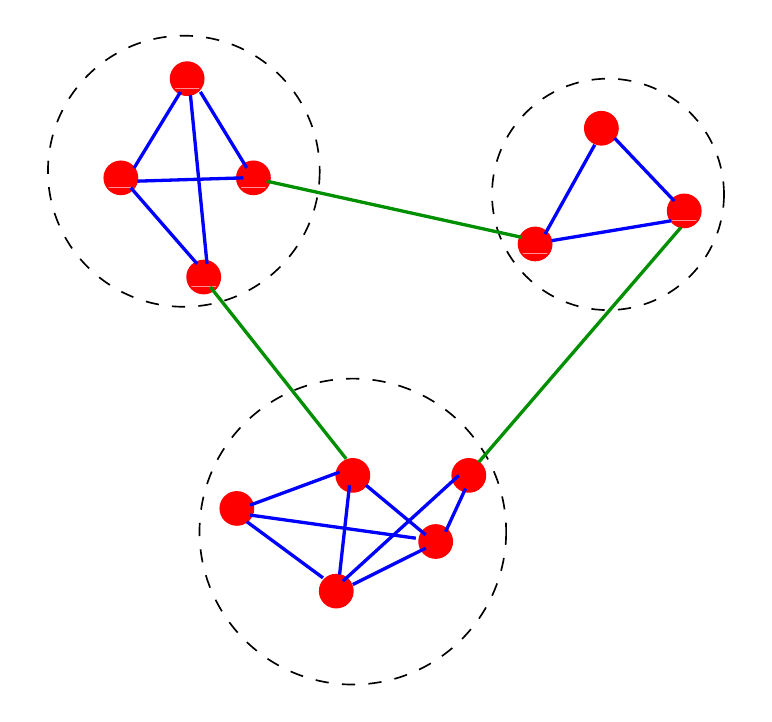
\includegraphics[width=8cm]{imagens/communities.png}
    \caption{Uma rede complexa simples composta por três comunidades.}
    \label{fig:communitystructure}
    \Fonte{\citeonline{Fortunato2010}}
\end{figure}

A identificação das comunidades que compõem uma rede provê a analistas uma visão mais sofisticada acerca de sua estrutura, fornecendo evidências sobre as funções dos grupos de vértices presentes na rede e de que forma estes grupos se comunicam. O processo também auxilia na análise da independência entre as comunidade da rede. Caso a rede não possua uma clara estrutura de comunidades, tal constatação caracteriza por si só uma importante informação sobre os aspectos da topologia da rede \cite{Newman2006}.

O estudo e a detecção de comunidades é de interesse prático em diversos domínios da ciência. Exemplos incluem a análise de páginas da \textit{web}, onde comunidades podem representar páginas que tratam de assuntos similares; a identificação de clientes com interesses similares, habilitando o desenvolvimento de sistemas de recomendação mais eficazes; o mapeamento de reações metabólicas e complexos de proteínas; o reconhecimento de indivíduos em redes criminosas; a identificação de componentes funcionais utilizados na percepção olfativa; entre outros \cite{Newman2006,Fortunato2010,Santiago2017}.

Segundo diversos autores, como \citeonline{Fortunato2007} e \citeonline{Newman2006}, a definição de comunidade não é totalmente exata e objetiva; geralmente, tem-se apenas uma noção intuitiva de seu conceito, envolvendo uma densidade elevada de ligações entre os vértices de uma comunidade (intra-comunidade) e poucas ligações entre vértices de comunidades diferentes (inter-comunidade). Cliques, definidos na Seção \ref{sec:graphfoundation}, são exemplos claros de comunidades; entretanto, dada sua raridade em redes complexas de tamanho razoável, considera-se que sua definição é muito rígida para ser adotada como um modelo prático de comunidade \cite{Fortunato2007}.

Sendo assim, algumas definições matemáticas foram desenvolvidas, as quais, em sua grande maioria, buscam avaliar a qualidade da divisão de uma rede complexa em comunidades. Com isso, torna-se possível identificá-las através de um processo de otimização matemática. Duas destas definições, que angariaram considerável popularidade na literatura, serão apresentadas nas próximas seções.

\subsubsection{Modularidade} \label{sec:modularity}

A otimização da função de Modularidade, desenvolvida por \citeonline{Newman2004}, é considerada a forma mais popular de efetuar o processo de detecção de comunidades por \citeonline{Fortunato2010}. A função é baseada no conceito da ausência da estrutura de comunidades em grafos aleatórios; sendo assim, define-se um ``modelo nulo''\footnote{Tradução livre de \textit{null model}}, que consiste em uma cópia da rede original porém com suas ligações redefinidas, buscando eliminar a estrutura de comunidades.

Após o estabelecimento do modelo nulo, computa-se a diferença entre a rede original, com seus vértices agrupados de alguma maneira, e seu modelo nulo. Caso não haja diferença, considera-se que o agrupamento dos vértices possui baixa qualidade -- isto é, não revela a estrutura de comunidades da rede. Por outro lado, se a diferença for elevada, então o agrupamento sob avaliação é tomado como um particionamento de alta qualidade da rede em suas comunidades \cite{Fortunato2010}.

O modelo nulo adotado com maior frequência envolve uma redefinição das ligações de forma a manter a distribuição de graus dos vértices da rede. Sendo assim, para um vértice $u$ qualquer, seu grau tende a ser igual ou similar no modelo nulo, porém o conjunto de vértices aos quais $u$ está conectado tende a ser totalmente diferente. Matematicamente, a probabilidade de dois vértices $u$ e $v$ estarem conectados no modelo nulo é dada por $\frac{k_uk_v}{2m}$, onde $k_u$ representa o grau do vértice $u$ e $m$ expressa o número de ligações presentes na rede. Com isso, define-se a função de Modularidade como:

\begin{equation}
    \label{eq:modularity}
    Q = \frac{1}{2m}\sum_{i=1}^{|V|}\sum_{j=1}^{|V|} \left [ \left ( A_{ij} - \frac{k_ik_j}{2m} \right ) \delta(C_i, C_j) \right ]
\end{equation}

\noindent onde $Q$ representa a função de Modularidade, $m$ representa o número de ligações da rede, $A$ expressa sua matriz de adjacências, $k_i$ simboliza o grau do vértice $i$ e a função $\delta(C_i, CC_j)$ possui valor 1 caso os vértices $i$ e $j$ pertençam à mesma comunidade e 0 caso contrário. A função $Q$ também pode ser trivialmente adaptada para grafos dirigidos e ponderados \cite{Fortunato2010}.

A detecção de comunidades através da otimização da função de Modularidade pertence à classe de problemas NP-difíceis, e portanto demanda esforço computacional extremamente elevado, sendo impraticável em redes complexas de tamanho razoável \cite{Brandes2008}. Para tratar desta característica, diversos métodos heurísticos foram desenvolvidos recentemente \cite{Blondel2008,Santiago2017,Nascimento2013,Agarwal2008,Pizzuti2008}.

Além disso, \citeonline{Fortunato2007b} identificaram que a detecção de comunidades por otimização da Modularidade apresenta um problema denominado ``resolução limite'', pelo qual a Modularidade tende a avaliar com maior qualidade agrupamentos de uma rede cujas comunidades são compostas por mais vértices. Sendo assim, o método é incapaz de identificar comunidades pequenas em redes razoavelmente grandes, mesmo quando tais comunidades são altamente coesas e esparsamente ligadas.

Um exemplo deste fenômeno é apresentado na Figura \ref{fig:ringofcliques}, onde uma rede composta por 16 cliques (cada qual contendo 4 vértices), conectados entre si por uma aresta, tem seu agrupamento ótimo consistindo em 8 comunidades de 2 cliques cada uma, ao invés do agrupamento esperado de 16 comunidades, com cada clique pertencendo à sua própria comunidade.

\begin{figure}[ht]
    \centering
    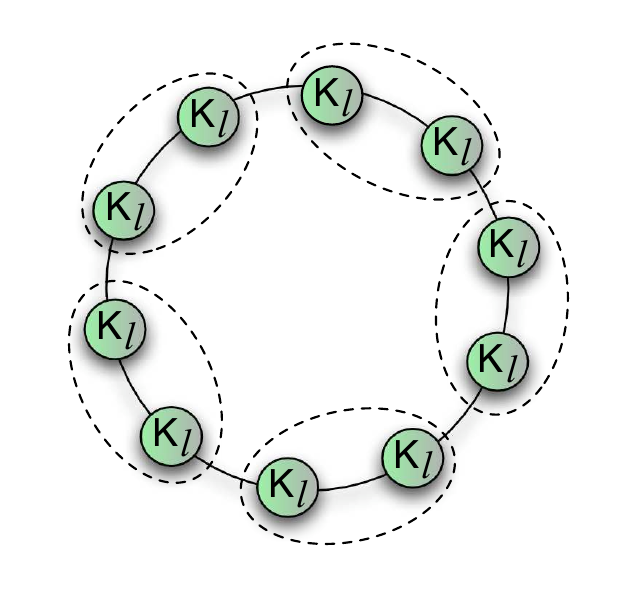
\includegraphics[width=9cm]{imagens/ring_of_cliques.png}
    \caption{Anel de cliques.}
    \label{fig:ringofcliques}
    \Fonte{\citeonline{Fortunato2010}}
\end{figure}

Uma função alternativa à Modularidade, desenvolvida com a intenção de contornar este problema, é apresentada na seção seguinte.

\subsubsection{Modularidade por Densidade} \label{sec:density}

Buscando solucionar os problemas associados à Modularidade apontados por \citeonline{Fortunato2007b}, \citeonline{Li2008} propuseram uma adaptação denominada Modularidade por Densidade. Nesta formulação, o número de vértices que compõem cada comunidade é utilizado para normalizar o resultado da equação, ao invés do número total de ligações do grafo como na Modularidade (conforme pode-se observar na Equação \ref{eq:modularity}.

Além disso, a utilização de um modelo nulo é substituída por um termo alternativo, que envolve o cômputo da diferença entre o número de ligações internas, com origem e destino em vértices da mesma comunidade, e ligações externas, com origem em vértices da comunidade atual e destino em vértices de outras comunidades \cite{Li2008,Santiago2017}. Em sua forma mais simples, a função de Modularidade por Densidade pode ser definida da seguinte maneira:

\begin{equation}
    \label{eq:density1}
    D = \sum_{C \in P} \left ( \frac{4|E_C| - \sum_{u \in C} k_u}{|C|} \right )
\end{equation}

\noindent onde $D$ simboliza a Modularidade por Densidade e $P$ representa o conjunto de comunidades, sendo cada comunidade expressa por $C$. Assim, para uma comunidade $C$ qualquer, $|C|$ indica o número de vértices que a compõem e $|E_C|$ representa o número de arestas internas à mesma. O termo $\sum_{u \in C} k_u$ consiste em um somatório dos graus dos vértices da comunidade, representando assim a densidade de ligações externas.

Usualmente, a Modularidade por Densidade é utilizada em sua variação paramétrica, que permite definir se é preferível identificar comunidades de tamanho pequeno ou grande. A Equação \ref{eq:density2} apresenta esta variação, onde o parâmetro $\lambda \in [0, 1]$ pode ser reduzido para encontrar comunidades menores ou aumentado para encontrar comunidades de porte maior. Caso o mesmo seja mantido em seu valor intermediário de 0,5, a função se comportará da mesma forma que a Equação \ref{eq:density1} \cite{Li2008,Santiago2017}. Nesta formulação, a função $g(C)$ representa o termo de ligações externas dado por $\sum_{u \in C} k_u$.

\begin{equation}
    \label{eq:density2}
    D_{\lambda} = \sum_{C \in P} \left ( \frac{4\lambda|E_C| - (2 - 2\lambda) (g(C) - 2|E_C|) }{|C|} \right )
\end{equation}

Assim como a Modularidade, a detecção de comunidades através da otimização da Modularidade por Densidade também demanda alto esforço computacional e, portanto, também é tipicamente utilizada em conjunto com métodos heurísticos. Exemplos incluem os algoritmos desenvolvidos por \citeonline{Gong2012}, \citeonline{Santiago2017} e \citeonline{KarimiMajd2015}.
\section{Coleta e Análise de Dados} \label{sec:data}

Esta seção apresenta uma revisão bibliográfica acerca do tópico de coleta de dados, descrevendo metodologias e diretrizes que visam assegurar um processo ético, replicável e livre de erros sistemáticos e vieses indevidos. Além disso, estratégias para realizar a análise dos dados coletados são levantadas e discutidas, com vista às particularidades deste estudo.

\subsection{Coleta de dados sociológicos} \label{sec:collection}

Pesquisas que investigam a influência e a relação entre pares, tanto em contextos educacionais quanto em outras situações, frequentemente utilizam questionários, onde cada participante é responsável por fornecer informações sobre seus pares. Em geral, busca-se compreender quão próximos os indivíduos se encontram socialmente, pois este fator impacta no poder de influência. Neste sentido, a escala da métrica pode ser tanto binária, onde apenas os contatos mais próximos são nomeados, quanto de múltiplos níveis, onde o grau de proximidade entre indivíduos é quantificado como um valor inteiro \cite{Rambaran2017,Blansky2013,Gremmen2017,Bellmore2010,Newman2003,Hymel1986,Schwartz2006}.

De acordo com \citeonline{Newman2003}, a coleta de dados sociológicos através de questionários ou entrevistas, onde os participantes fornecem informações de forma direta e opinativa, é um processo trabalhoso e sujeito a erros. Nestas situações, o tamanho das redes sociais investigadas tende a ser consideravelmente limitado, devido ao aspecto manual da coleta de dados; além disso, as informações fornecidas pelos participantes são invariavelmente subjetivas e, portanto, profundamente sujeitas a vieses.

Assim, ocorrências recentes de significância limitada e breve (uma discordância em uma conversa ou o recebimento de um presente, por exemplo) podem causar um impacto maior do que o apropriado sobre a visão de um participante acerca de outro. No entanto, segundo \citeonline{Newman2003}, as limitações envolvendo esta metodologia de coleta de dados são geralmente compreendidas e aceitas pela comunidade científica.

Em outro trabalho, \citeonline{Newman2010} sugere que a coleta de dados por meio de questionamentos aos próprios participantes é o método mais comum de acúmulo de informações relacionadas a redes sociais; além disso, o autor comenta que as incertezas e fragilidades associadas a este método se fazem presentes em praticamente todas as pesquisas de cunho social, não sendo exclusivas aos estudos que tratam da análise de redes complexas.

\citeonline{Marsden1990} fornece uma revisão acerca do tópico, apresentando diversos pontos de vista e sintetizando trabalhos que seguem a metodologia. O autor, em termos gerais, toma uma perspectiva positiva, comentando que, apesar das incertezas, dados coletados por questionários e entrevistas são indubitavelmente úteis e importantes, desde que suas limitações sejam observadas.

Tratando de métodos para aprimorar a acurácia dos resultados de questionários e entrevistas, sugere-se: (i) comparação com um padrão conhecido, através do uso de dados de catálogos e de pesquisas já realizadas; (ii) análise de reciprocidade, dado que relações mútuas sugerem um padrão e não apenas uma observação ao acaso; e (iii) teste-reteste, onde a pesquisa é realizada em dois pontos no tempo, sendo esperado que a estrutura geral da rede mantenha-se relativamente estável. No entanto, nenhum método é capaz de garantir a confiabilidade total dos resultados \cite{Marsden1990}.

Entre outras metodologias para coleta de dados relacionados a redes sociais, tem-se: (i) análise de colaborações, onde laços são estabelecidos entre atores que participaram de alguma atividade em conjunto -- por exemplo, atores que participaram do elenco de um mesmo filme ou cientistas que colaboraram na escrita de um artigo; (ii) compilação de catálogos, onde eventos registrados são analisados pelo pesquisador, possibilitando a reconstrução da rede a partir de padrões de interação como troca de correspondências, chamadas telefônicas, laços familiares e, recentemente, relacionamentos por mídias sociais como Facebook; (iii) observação direta, onde o pesquisador apenas observa um grupo de indivíduos por um período de tempo, tomando nota de suas interações e registrando-as de acordo com seu ponto de vista \cite{Marsden1990,Newman2004,Newman2010}.

\subsubsection{Considerações Éticas e Diretrizes} \label{sec:ethics}

A coleta de dados sociológicos através de questionários, visando a reconstrução de redes sociais, se trata de um procedimento onde o anonimato total é impraticável, tendo em vista que (i) os participantes devem identificar seus contatos de alguma maneira, seja preenchendo nomes em meio físico ou digital ou escolhendo-os de uma lista de indivíduos predefinida, e (ii) o processo de reconstrução pressupõe que seja possível identificar os respondentes, pois representam a extremidade de origem de cada laço social  \cite{Marsden1990}. Naturalmente, é possível implementar um estágio de anonimização no tratamento dos dados, eliminando informações de identificação pessoal; a Seção \ref{sec:anonymization} discorre em detalhes sobre o tema, apresentando algumas metodologias de implantação.

Boa parte dos trabalhos publicados na área que incluem a aplicação de um questionário abordam a privacidade de dados de alguma maneira. Tipicamente, ao lidar com crianças e adolescentes, os pesquisadores consultam os pais dos participantes, solicitando que os mesmos assinem um termo de consentimento caso permitam que seus filhos façam parte da pesquisa; o termo assegura a confidencialidade das respostas e estabelece que, por opção tanto dos pais quanto dos filhos, a participação pode ser encerrada a qualquer momento \cite{Hymel1986,Schwartz2006,Bellmore2010,Rambaran2017}.

De fato, conforme \citeonline{DeLeeuw2008} comentam, diversos regulamentos e códigos de ética em pesquisa demandam que, entre outros itens, os estudos: (i) obtenham consentimento informado, onde os participantes\footnote{Caso estejam abaixo de uma certa idade, determinada pelo país em que vivem, o consentimento deve ser obtido dos pais dos participantes.} devem estar ciente sobre propósitos da pesquisa, seus riscos e seus benefícios; (ii) mantenham a confidencialidade das respostas, utilizando-os apenas para os propósitos estabelecidos e evitando que terceiros não autorizados obtenham acesso aos dados; e (iii) permitam que os participantes se recusem a cumprir qualquer ação proposta e que possam abandonar a pesquisa a qualquer instante.

O Comitê de Ética em Pesquisa da UNIVALI estabelece algumas normas e diretrizes para pesquisas envolvendo seres humanos. Quanto à utilização de dados de sujeitos investigados, determina-se que \cite{Univali2002}:

\begin{alineas}
    \item apenas projetos aprovados pelo Comitê são autorizados a acessar bases de dados da Instituição;
    \item os investigados deverão fornecer Consentimento Livre e Esclarecido ou, caso isso seja impossível ou desnecessário, os investigadores deverão utilizar um Termo de Compromisso de Utilização de Dados;
    \item o anonimato dos investigados e a confidencialidade de seus dados devem ser mantidos por todos os envolvidos;
    \item os dados poderão ser usados somente para cumprir os propósitos do projeto aprovado pelo Comitê.
\end{alineas}

\subsection{Anonimização} \label{sec:anonymization}

\citeonline{Raghunathan2013} define a anonimização como o processo de remoção de informações de identificação pessoal de dados sensíveis, preservando o formato e o tipo dos dados. Dependendo da técnica, a saída do processo de anonimização pode ser realístico, assemelhando-se a um dado real porém sem nenhuma associação ao original, ou aleatório, onde o dado é substituído por uma sequência aleatória de caracteres ou números; além disso, o resultado pode ou não ser determinístico, onde a mesma entrada sempre gera a mesma saída.

Além de ser utilizada para contemplar obrigações impostas por leis, normas e códigos de ética, conforme descrito na Seção \ref{sec:ethics}, a anonimização também reduz a probabilidade de situações litigiosas, onde o acesso a dados sigilosos por indivíduos ou grupos mal-intencionados pode causar prejuízos ou desconfortos de qualquer espécie aos indivíduos que forneceram suas informações \cite{Raghunathan2013}.

Estas consequências negativas podem variar de constrangimentos temporários (advindos, por exemplo, de informações relacionadas a comportamentos pessoais delicados) a danos sérios à imagem individual, quando se trata de pesquisas envolvendo informações ilícitas, criminais ou potencialmente degradantes \cite{DeLeeuw2008}. Além disso, primariamente em contextos empresariais, há a possibilidade de danos financeiros significativos, podendo acarretar em endividamento e falência de organizações \cite{Raghunathan2013}.

Segundo \citeonline{Raghunathan2013}, as principais técnicas disponíveis para a implementação do processo de anonimização em tipos de dados genéricos\footnote{Existem métodos para tipos específicos, como datas e números; por brevidade, estes foram omitidos.} são:

\begin{alineas}
    \item Criptografia: utilizada principalmente quando a confidencialidade e integridade dos dados são prioritárias, não existindo a necessidade de manter a aparência realística no valor de saída. Divide-se em:
    \begin{alineas}
        \item Chave simétrica: método reversível onde a mesma chave é utilizada tanto para criptografar quanto para descriptografar;
        \item Chave pública: similar ao método simétrico, porém há um par de chaves (pública e privada) onde o dado é criptografado com uma e descriptografado com outra;
        \item \textit{Hashing}: método irreversível e determinístico que transforma o valor de entrada em uma sequência de caracteres de comprimento fixo.
    \end{alineas}
    \item Substituição: o dado é substituído por outro valor, sendo gerado aleatoriamente ou advindo de um mapeamento predefinido. Esta técnica pode ser aplicada caractere a caractere ou em grupos, como palavra a palavra;
    \item Ocultação de caracteres: cada item do dado é substituído por um caractere especial, como X ou asteriscos, mantendo seu comprimento original. Frequentemente utilizado para ocultar números de cartão de crédito;
    \item Embaralhamento: considerando uma tabela de dados, embaralha-se as linhas de uma mesma coluna da tabela, mantendo as demais colunas intactas;
    \item Anulação: nesta técnica, simplesmente substitui-se o dado sensível por um valor nulo ou em branco.
\end{alineas}

Destas técnicas, apenas a criptografia e a substituição podem ser utilizadas de forma determinística (repetível). Tal característica é necessária quando se deseja manter a integridade relacional entre múltiplos bancos de dados e, por extensão, quando é necessário associar dados advindos de bases de dados diferentes \cite{Raghunathan2013}.

\subsection{Métodos de Análise} \label{sec:analysis}

\citeonline{Borgatti2013} compreendem que a análise de redes sociais pode ser dividida em dois tipos: (i) aplicada, onde estuda-se a estrutura da rede, extraindo-se as métricas apropriadas, e subsequentemente os resultados são interpretados de forma a possibilitar o desenvolvimento de alguma espécie de intervenção, inexistindo qualquer investigação acerca das correlações entre as variáveis sob estudo; e (ii) básica, onde busca-se identificar e explicar a correlação entre duas ou mais variáveis, sendo que tipicamente caracteriza-se comportamentos observados nos indivíduos como causas ou efeitos de métricas extraídas da rede.

A análise do tipo básico serve como fundamentação para estudos aplicados, e é utilizada em grande parte dos trabalhos científicos publicados na área \cite{Borgatti2013}. Por ser uma pesquisa descritiva, onde não haverá nenhum tipo de intervenção aplicado sobre o ambiente ou sobre os indivíduos estudados, este trabalho fará uso do tipo básico de análise de redes sociais.

Ao utilizar-se de métricas da rede (como a centralidade, descrita na Seção \ref{sec:centrality}) para explicar comportamentos existentes ou predizer sua ocorrência, tem-se uma análise básica sob a perspectiva da rede como \emph{causa}. Nestes estudos, compreende-se que os comportamentos observados na população são resultantes da estrutura da rede social subjacente; matematicamente, variáveis da rede são classificadas como independentes e da população como dependentes.

\citeonline{Borgatti2013} exemplificam este subtipo de análise com a utilização da centralidade dos atores de uma rede social corporativa (onde laços representam confiança) como variável preditiva da probabilidade de seleção para promoção dentro da organização. O trabalho de \citeonline{Blansky2013}, descrito em detalhes na Seção \ref{sec:blansky}, ilustra claramente o estudo da rede como causa: em sua análise estatística, os autores buscaram inferir uma função que mapeia variáveis derivadas da estrutura da rede para a mudança no desempenho acadêmico de estudantes.

Por outro lado, é possível investigar as formas com que o comportamento individual ou coletivo age sobre a estrutura das redes sociais. Nesse caso, tem-se uma perspectiva da rede como \emph{efeito}, sendo as variáveis da mesma vistas como independentes e aquelas extraídas dos indivíd2uos (ou do grupo) vistas como dependentes. Sendo assim, análises associadas com este subtipo tipicamente se concentram em caracterizar a influência de fatores socialmente significativos -- como raça, gênero, idade e renda -- sobre a formação ou rompimento de laços entre indivíduos \cite{Borgatti2013}.

Nestas análises, considera-se dois aspectos principais: (i) preferência, onde o indivíduo forma ou rompe laços livremente, de acordo com suas opiniões, motivações e vontades, sendo a homofilia (descrita na Seção \ref{sec:socialnetworks}) um fator que causa impacto significativo neste aspecto; e (ii) oportunidades e restrições, onde o indivíduo modifica ou mantém seus laços de acordo com as limitações impostas a ele pelo ambiente em que está inserido -- por exemplo, ao analisar-se a rede social de uma escola composta predominantemente por homens, o conjunto de contatos imediatos de qualquer indivíduo conterá uma proporção muito maior de homens do que de mulheres \textit{(ibidem)}.

\subsection{Visualização} \label{sec:visualization}

Segundo \citeonline{Bondy1976}, o termo ``grafo'' advém da capacidade dos mesmos de serem representados de forma gráfica, onde vértices são indicados por pontos ou círculos (ou, menos frequentemente, por outras formas geométricas) e ligações são representadas por linhas ou curvas. A diagramação ilustrada de um grafo, denominada \emph{visualização}, fornece uma compreensão rápida e intuitiva acerca de suas propriedades estruturais, possibilitando a realização de uma análise qualitativa que, em geral, revela características difíceis de serem obtidas de forma quantitativa. Assim, a visualização é frequentemente utilizada em estudos envolvendo a análise de redes complexas, independentemente da metodologia de pesquisa do trabalho \cite{Borgatti2013,Bondy1976}.

Entretanto, no sentido geral, grafos não carregam consigo qualquer informação precisa acerca de sua visualização apropriada. Portanto, não há uma forma única de produzir a ilustração de um grafo, fazendo com que as posições de seus vértices no espaço possam ser determinadas de forma arbitrária \cite{Bondy1976}. Apesar disso, \citeonline{Borgatti2013} especificam que a disposição dos vértices do grafo é o aspecto mais importante de sua visualização, por influenciar diretamente as interpretações de analistas sobre suas características estruturais. A Figura \ref{fig:vizcomparison} demonstra esta importância, onde a mesma rede complexa tem seus vértices dispostos de forma aleatória (à esquerda) e com base em um algoritmo de visualização (à direita), onde esta última revela uma estrutura de duas comunidades.

\begin{figure}[ht]
    \centering
    \begin{subfigure}{0.49\textwidth}
        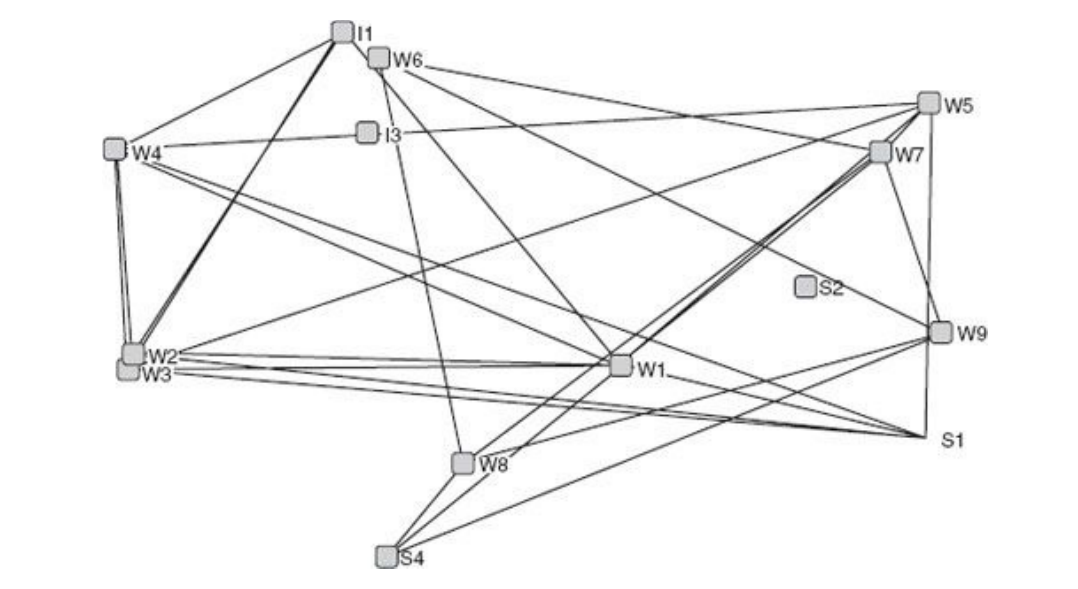
\includegraphics[width=\linewidth]{imagens/randomlayout.png}
        \caption{Aleatória} \label{fig:viza}
    \end{subfigure}
    %\\
    \vspace*{0.35cm}
    \begin{subfigure}{0.49\textwidth}
        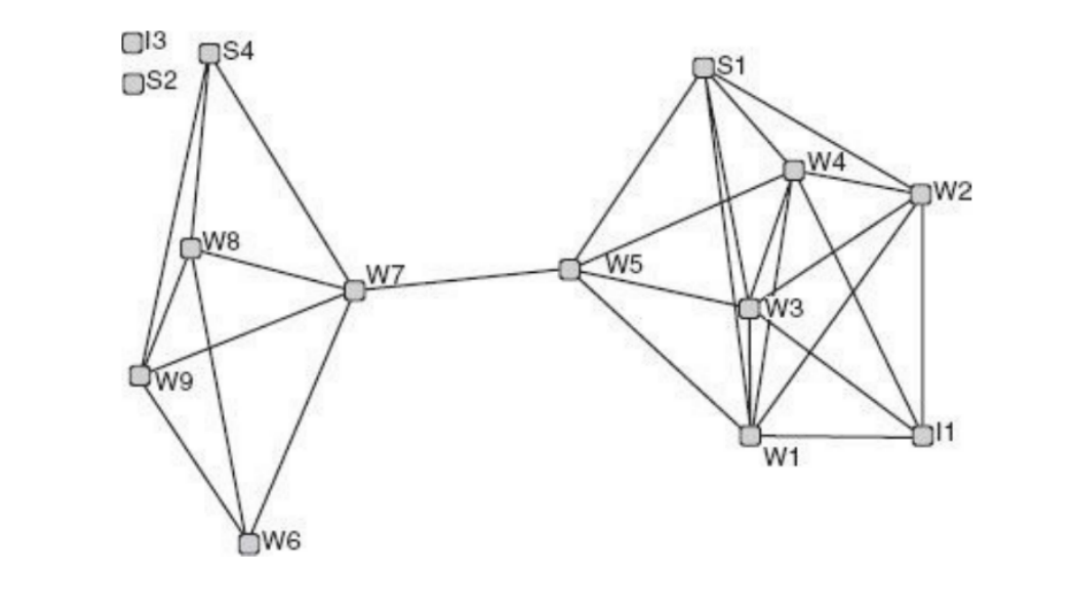
\includegraphics[width=\linewidth]{imagens/goodlayout2.png}
        \caption{Baseada em algoritmo} \label{fig:vizb}
    \end{subfigure}
    \vspace*{0.3cm}
    \caption{Comparação de visualizações de uma mesma rede complexa.}
    \label{fig:vizcomparison}
    \Fonte{Adaptado de \citeonline{Borgatti2013}.}
\end{figure}

% Referenciar PCA???
\citeonline{Borgatti2013} enumeram três estratégias para produzir visualizações de grafos: (i) gráfico de dispersão, onde atributos dos vértices são utilizados para determinar as suas coordenadas no plano cartesiano; (ii) redução de dimensionalidade, através de técnicas como análise de componentes principais, onde matrizes de associação entre vértices (contendo, por exemplo, distâncias ou correlações entre atributos) são mapeadas para coordenadas, aproximando os vértices de acordo com sua similaridade; e (iii) algoritmos de disposição de grafos, que são desenvolvidos especialmente para a tarefa de visualização e subdividem-se em vários tipos, como iterativos ou baseados em otimização matemática. \citeonline{Herman2000} fornecem uma revisão acerca de algoritmos de disposição, apontando suas características, vantagens e desvantagens.

Além disso, é possível aprimorar a interpretabilidade da visualização de grafos empregando artifícios como variação de cores, formas, tamanhos e espessuras. Por exemplo, pode-se utilizar a centralidade (discutida na Seção \ref{sec:centrality}) de cada vértice para determinar seu tamanho, modificar a espessura das ligações de acordo com seu peso, utilizar setas para indicar a direção dos arcos, entre outras opções \cite{Borgatti2013}.

\subsection{Análise Estatística} \label{sec:correlation}

A visualização de grafos, apesar de ser uma ferramenta de análise poderosa, está restrita ao domínio qualitativo e, portanto, está sujeita a interpretações e questões subjetivas, especialmente ao levar-se em conta as incertezas envolvendo a disposição dos vértices. Sendo assim, abordagens quantitativas, que apropriam-se de métodos estatísticos clássicos, também angariam considerável interesse na comunidade científica, por serem capazes de fornecer uma perspectiva objetiva e confirmatória acerca dos dados sob análise \cite{Atieno2009,Borgatti2013}.

No entanto, técnicas estatísticas clássicas assumem que os dados apresentam algumas características que não estão presentes em redes sociais, como a independência entre observações (afinal, sabe-se que existem processos de influência entre atores, conforme comentado na Seção \ref{sec:socialinfluence}) e a existência de uma distribuição estatística subjacente. Sendo assim, torna-se necessário realizar adaptações destas técnicas, visando habilitar seu uso de forma adequada em grafos \cite{Borgatti2013}. Conforme descrito na Seção \ref{sec:analysis}, análises básicas tem como objetivo principal identificar relações entre variáveis; para tanto, utiliza-se principalmente testes de hipótese, métodos de regressão (como a regressão linear) e métricas de correlação (como a de Pearson) \cite{DeNooy2005,Borgatti2013}.

\citeonline{Borgatti2013} sugerem a utilização de um método conhecido como \emph{teste de permutação}, que consiste em uma extensão a testes estatísticos clássicos. Testes de permutação consideram todos os resultados possíveis de um experimento, produzindo amostras de maneira aleatória; posteriormente, compara-se o valor de correlação obtido da amostra original com a distribuição de correlações das amostras aleatórias geradas. Com isso, calcula-se a proporção de amostras aleatórias que apresentaram correlação igual ou superior à original. Caso esta proporção seja inferior a um valor predeterminado (geralmente 5\%), então define-se que a relação entre as variáveis sob investigação é estatisticamente significante.
% com isso, a necessidade de independência é anulada.

Além disso, a existência de dois tipos de componentes em grafos -- vértices e ligações -- faz com que seja necessário utilizar metodologias adequadas ao nível de análise pretendido, de acordo com a hipótese que deseja-se testar. \citeonline{Borgatti2013} enumeram quatro níveis: (i) monádico, onde relaciona-se variáveis pertencentes exclusivamente a vértices; (ii) diádico, onde a análise é realizada entre pares de vértices, considerando características dos laços (imediatos ou não); (iii) misto, onde busca-se associar variáveis monádicas com diádicas (por exemplo, centralidade com amizades); e (iv) global, onde analisa-se variáveis que dizem respeito ao grafo como um todo (por exemplo, densidade e modularidade).

Para os níveis monádicos e globais, pode-se empregar técnicas estatísticas naturalmente, bastando utilizá-las juntamente com testes de permutação. No entanto, análises envolvendo díades (níveis diádicos e mistos) apresentam dificuldades significativas, pois as variáveis assumem um formato matricial, seguindo a estrutura da matriz de adjacências (discutida na Seção \ref{fig:networkDefs}). Como as técnicas estatísticas clássicas estão aptas para lidar apenas com dados vetoriais, métodos específicos são necessários.

Um destes métodos é a família de estratégias QAP (\textit{Quadratic Assignment Procedure}\footnote{Tradução livre: Procedimento de Atribuição Quadrático}), desenvolvida por \citeonline{Hubert1976} e estudada no contexto de redes sociais por \citeonline{Krackhardt1988}. A técnica, disponível em forma de análise de correlação e regressão na aplicação UCINET \cite{Borgatti2013}, é capaz de inferir associações entre matrizes de dados, e portanto pode ser empregada em níveis de análise diádicos. No caso do nível misto, existem estratégias para converter o vetor de dados monádico em uma matriz, possibilitando aplicação da técnica QAP \cite{Borgatti2013}, sendo possível também converter a matriz de dados diádica em um vetor, permitindo o uso de técnicas clássicas \cite{Blansky2013}.

\subsection{SIENA} \label{sec:siena}

A metodologia SIENA (\textit{Simulation Investigation for Empirical Network Analysis}\footnote{Tradução livre: Investigação de Simulações para Análise Empírica de Redes}), proposta por \citeonline{Snijders2001}, consiste em uma abordagem baseada em atores voltada para a análise de dados de redes sociais coletados de forma longitudinal; ou seja, onde tem-se instâncias de uma mesma rede de indivíduos em diferentes pontos no tempo.

A metodologia, em linhas gerais, busca simular o comportamento de processos sociais reais através de uma cadeia de Markov de tempo contínuo, onde o único evento passível de ocorrência em cada instante da simulação é a formação ou rompimento de uma ligação entre um par de vértices. Sendo assim, o modelo busca decompôr as mudanças ocorridas na rede social de uma coleta de dados para a próxima em passos simples, de apenas um evento. A frequência de execução de passos na simulação é especificada por uma função, que consiste em um parâmetro do modelo \cite{Borgatti2013}.

Por se tratar de uma abordagem baseada em atores, a simulação realizada pelo SIENA tem como ponto chave o processo de decisão individual de cada de ator da rede social, onde a opção por formação ou rompimento de ligações é guiada por uma função de avaliação definida pelo analista. Esta função pode levar em consideração atributos monádicos, diádicos e globais; com isso, é possível extrair inferências acerca destas variáveis, tornando o modelo altamente flexível e aplicável a uma grande gama de contextos (exemplos incluem os trabalhos de \citeonline{Rambaran2017} e \citeonline{Gremmen2017}, descritos na próxima seção). Entretanto, devido à complexidade inerente ao processo de simulação, podem existir dificuldades no tocante à interpretação dos resultados produzidos pelo modelo \textit{(ibidem)}.

% provavelmente vai ter que mudar \ref{sec:rambaran}
% já mudei



\section{Trabalhos Relacionados} \label{sec:relatedwork}

Nesta seção, são apresentados três trabalhos recentes com objetivos, materiais e métodos relacionados com o presente estudo. Os trabalhos incluem a pesquisa de \citeonline{Blansky2013}, que investigaram a dinâmica de contágio social entre estudantes do ensino médio, correlacionando a influência de amizades imediatas com a evolução das notas dos alunos; o estudo de \citeonline{Rambaran2017}, que analisou a influência de amizades sobre notas e frequência durante dois anos, com atenção às diferenças entre popularidade e aceitação; e a publicação de \citeonline{Gremmen2017}, cuja metodologia assemelha-se à de \citeonline{Rambaran2017}, porém com maior ênfase na diferenciação dos processos de seleção e influência de amizades sobre o desempenho acadêmico.

Ao término da seção, apresenta-se uma análise comparativa entre os três trabalhos selecionados e o presente, fornecendo uma visão geral acerca das diferenças e similaridades nas abordagens.

\subsection{Spread of Academic Success in a High School Network} \label{sec:blansky}

O estudo de \citeonline{Blansky2013} envolveu a análise do processo de disseminação de comportamento em alunos de uma escola dos Estados Unidos, investigando o impacto deste processo nas notas dos estudantes ao longo do tempo. A pesquisa foi realizada na escola Maine-Endwell High School (Nova Iorque) no ano de 2011, sobre estudantes da turma do décimo primeiro estágio\footnote{A turma é denominada \textit{eleventh grade} nos Estados Unidos, sendo equivalente ao segundo ano do Ensino Médio no Brasil.}.

A amostra utilizada no estudo foi composta por 158 alunos, onde cada integrante teve de avaliar cada um de seus colegas em termos da proximidade social entre os dois, em uma escala de: (i) melhor amigo; (ii) amigo; (iii) conhecido; (iv) não nos conhecemos\footnote{No artigo original, os termos utilizados foram, em ordem, \textit{best friend}, \textit{friend} e \textit{acquaintance}.}. O questionário também perguntava se os alunos pertenciam à mesma família, porém esta informação não foi utilizada para compôr a rede complexa que modela os alunos amostrados. Juntamente com este dado, os autores obtiveram, diretamente da escola, as notas médias de cada aluno em dois pontos no tempo: na data de aplicação do questionário e exatamente um ano depois da data.

Com ambas as fontes de dados associadas, os autores construíram um modelo estatístico utilizando o método de regressão linear, identificando uma correlação positiva e estatisticamente significante entre o aumento do desempenho acadêmico de alunos e a diferença de suas notas com a de seus amigos; assim, alunos cujos amigos possuem notas superiores às suas tendem a tirar notas cada vez maiores.

Para eliminar a influência de fatores indevidos, os autores construíam um modelo nulo da rede complexa, seguindo a mesma linha de raciocínio da Modularidade (Seção \ref{sec:modularity}) de \citeonline{Newman2004}. Após analisar 500 instâncias do modelo nulo, os autores observaram que o grau de correlação diminuiu significativamente em todas elas, confirmando que notas dos amigos imediatos dos estudantes de fato causam impacto em seu desempenho.

\subsection{Academic Functioning and Peer Influences: A Short-Term Longitudinal Study of Network--Behavior Dynamics in Middle Adolescence} \label{sec:rambaran}

Em sua pesquisa, \citeonline{Rambaran2017} analisaram a relação entre laços de amizade e o funcionamento acadêmico de adolescentes, o qual é composto tanto pelas notas médias quanto pelo absenteísmo dos estudantes. Como objetivos principais, os autores elencaram: (i) verificar relação entre funcionamento acadêmico e processos de seleção de influência de pares; (ii) verificar a direção da operação dos processos de seleção e influência; e (iii) analisar o impacto da popularidade e da aceitação entre amigos sobre a associação entre influência de pares e funcionamento acadêmico.

Foi realizada uma amostragem sobre uma escola pública de ensino médio, localizada no sul da Califórnia, onde 342 dos 1200 alunos matriculados participaram do estudo. A coleta de dados foi realizada de forma longitudinal, iniciando em setembro de 1997 e sendo concluída em junho de 1999. Quatro repetições foram realizadas, com intervalos de cerca de 6 meses, sendo que os mesmos indicadores foram utilizados em todas as instâncias.

Assim como no trabalho de \citeonline{Blansky2013}, os autores utilizaram um formulário onde os alunos avaliam seus colegas; porém, devido ao elevado número de integrantes, cada aluno avaliou apenas 50 colegas, escolhidos aleatoriamente. O formulário foi composto por duas perguntas por indivíduo: ``quão popular você considera este aluno?'' e ``quanto você gosta de bater papo\footnote{A expressão inglesa \textit{hang out} foi utilizada no formulário original.} com este aluno?''. Ambas as perguntas possuiam uma escala no intervalo de 1 a 5. Além disso, cada aluno recebeu uma folha com os nomes de todos os participantes, sendo solicitado que circulassem os nomes de todos os amigos próximos. Foi associado a cada respondente seu histórico de notas médias e o número de faltas não justificadas.

No estágio de análise de resultados, os autores utilizaram o sistema SIENA, descrito em detalhes na Seção \ref{sec:siena}, que fornece um conjunto de ferramentas para análise longitudinal de redes sociais, envolvendo um modelo de simulação baseado em atores. Para contemplar o processo de seleção de pares, os autores utilizaram as nomeações de amigos próximos por escrito; para o processo de influência, foi analisada a tendência das notas de pares se tornarem mais próximas ao longo do tempo.

Como conclusões, os autores reportaram que indivíduos que formam laços de amizade com alunos que demonstram alto desempenho tendem a tirar notas mais altas, enquanto aqueles que tornam-se amigos de alunos de baixo desempenho tendem a faltar mais e, por consequência, tirar notas mais baixas. Além disso, indivíduos com baixa frequência tendem a receber menos menções de amizade próxima, principalmente de alunos com alto desempenho. Indivíduos com alta popularidade causaram impacto apenas em amizades mútuas e apenas sobre frequência, enquanto alunos com alta taxa de aceitação (dada pelo indicador ``gosta de bater papo'') causaram impacto tanto em amizades unilaterais quanto mútuas e tanto em notas quanto frequência.
% Esclarecer que unilateral = díade e mútua = tríade

\subsection{First Selection, Then Influence: Developmental Differences In Friendship Dynamics Regarding Academic Achievement} \label{sec:gremmen}

Em um estudo consideravelmente similar ao de \citeonline{Rambaran2017}, \citeonline{Gremmen2017} exploram a relação entre os processos de seleção e influência e o desempenho de estudantes em duas escolas da Holanda. Os autores selecionaram alunos na fase de transição entre o ensino fundamental e o ensino médio holandês, o qual é baseado em três trilhas de estudo; com isso, foi possível capturar com maior acurácia o processo de seleção de pares (pois o aluno é inserido em um ambiente com um conjunto de colegas diferente), diferenciando-o da influência, que se dá após laços de amizade terem sido formados.

Como objetivos do trabalho, os autores buscaram investigar duas hipóteses: (i) a probabilidade de dois indivíduos se tornarem amigos aumenta conforme maior for a similaridade de seu desempenho acadêmico; e (ii) o desempenho acadêmico de amigos tende a se tornar mais similar ao longo do tempo. A primeira trata do processo de seleção, enquanto a segunda trata da influência.

Quanto aos dados, o estudo considerou os dois primeiros anos do ensino médio holandês, envolvendo um total de 556 participantes. A coleta de dados foi realizada em 6 datas, estendendo-se de outubro de 2011 a abril de 2013. Os indicadores utilizados foram: notas médias, melhores amizades na classe (por nomeação; ou seja, 0 ou 1), assiduidade com deveres de casa (1 a 10) e satisfação com a escola (1 a 4). O primeiro foi obtido diretamente com as escolas, enquanto os demais foram coletados através de um questionário.

Assim como \citeonline{Rambaran2017}, os autores utilizaram o sistema SIENA para analisar os dados coletados. As notas foram divididas em três grupos temáticos: (i) idioma, composto pelas disciplinas de holandês e inglês; (ii) exatas/ciências, composto por matemática e biologia; e (iii) social, composto por história e geografia.

Em sua análise, os autores identificaram que, no primeiro ano do ensino médio holandês, a seleção de amizades é afetada significativamente pela similaridade de notas no mesmo grupo temático, mas não foi possível identificar o processo de influência. No segundo ano, entretanto, o comportamento inverso foi observado: a influência de amizades apresentou grande efeito no desempenho acadêmico, mas a seleção se deu de forma independente da similaridade de notas.

Além disso, alunos com alto desempenho tendem a evitar formar laços de amizade com colegas com baixo desempenho; no sentido oposto, o comportamento também pode ser observado, mas com menos proeminência. Por fim, tanto a seleção quanto a influência se mostraram mais evidentes quando notas do mesmo grupo temático foram consideradas, ao invés da média geral.

\subsection{Análise Comparativa} \label{sec:relatedcomparison}

Esta seção apresenta uma análise comparativa entre os trabalhos de \citeonline{Blansky2013}, \citeonline{Rambaran2017} e \citeonline{Gremmen2017}, expondo de forma sintética suas similaridades, diferenças e evidenciando a maneira com que o presente estudo se relaciona com eles.

\begin{quadro}[ht]
    \caption{Comparativo entre trabalhos relacionados}
    \label{board:related}
    \fontsize{10}{12}\selectfont
    \def\arraystretch{1.25}
    \begin{tabularx}{\textwidth}{|c|Y|c|c|c|}
        \hline
        \textbf{Trabalho} & \textbf{Participantes} & \textbf{Escala de amizade} & \textbf{Período de estudo} & \textbf{Validação}
        \\ \hline
        \citeonline{Blansky2013} & 2º ano do ensino médio, EUA & 0 a 3 & 1 ano & Modelo nulo
        \\ \hline
        \citeonline{Rambaran2017} & 1º e 2º anos do ensino médio, EUA & 1 a 5; 0 ou 1 & 2 anos & SIENA
        \\ \hline
        \citeonline{Gremmen2017} & 1º e 2º anos do ensino médio, Holanda & 0 ou 1 & 2 anos & SIENA
        \\ \hline
        Este estudo & Ensino superior, Brasil & 0 a 5 & 1 ano & Modelo nulo
        \\ \hline
    \end{tabularx}
\end{quadro}

Todos os trabalhos descritos realizam a reconstrução das redes sociais através da aplicação de questionários, respondidos pelos próprios alunos, cada um com uma escala própria. \citeonline{Rambaran2017} utilizam duas questões relacionadas a amizade, conforme descrito na Seção \ref{sec:rambaran}; portanto, na tabela, são apresentadas as escalas referentes às questões ``bater papo'' e ``amigos mais próximos'', respectivamente. Quanto ao período de estudo, no caso do trabalho de \citeonline{Blansky2013} e do presente, apenas uma coleta de dados sobre amizade via questionário será realizada, porém um histórico extenso de notas será levado em consideração.
  \clearpage
\chapter{Projeto} \label{sec:project}

Nesta seção, apresenta-se a metodologia proposta para a investigação das perguntas de pesquisa estabelecidas no presente estudo, buscando-se analisar, através da aplicação do arcabouço teórico das áreas de Teoria dos Grafos, Redes Complexas e Análise de Redes Sociais, o impacto do círculo social de estudantes do ensino superior sobre seu desempenho acadêmico. Para tanto, o projeto divide-se em três etapas: (i) coleta de dados, compreendendo a elaboração e aplicação do instrumento de pesquisa, assim como a coleta de informações referentes às notas da população pesquisada e a anonimização dos dados; (ii) reconstrução e associação, que aborda a transformação dos dados coletados em redes complexas e a reconciliação das duas fontes de dados; e (iii) análise, que busca extrair inferências a partir dos dados combinados e responder concretamente às perguntas de pesquisa levantadas.

Na Figura \ref{fig:process}, apresenta-se uma visão geral sobre a metodologia proposta, incluindo as três etapas enumeradas. Atenção especial é dada aos processos que lidam com dados sensíveis (expressos em vermelho).

\begin{figure}[ht]
    \centering
    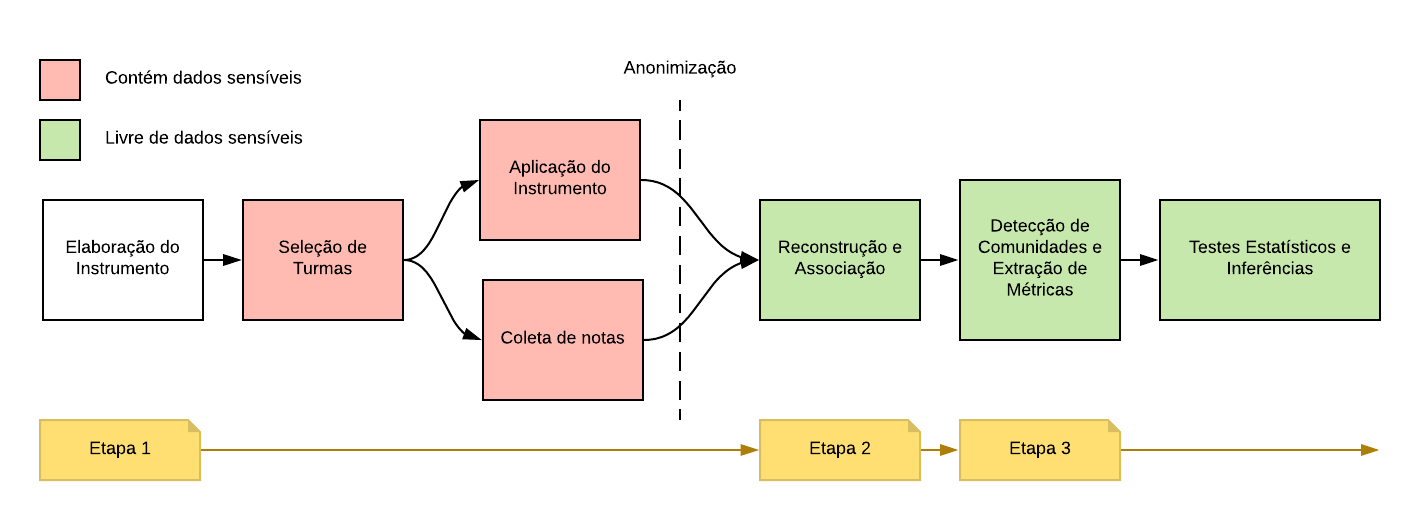
\includegraphics[width=\textwidth]{imagens/fluxo_ttc.png}
    \caption{Fluxo de atividades.}
    \label{fig:process}
    \Fonte{o autor.}
\end{figure}

\section{Coleta de Dados} \label{sec:datacollection}

A etapa de coleta de dados compreende os procedimentos que serão empregados para identificar, coletar e armazenar informações referentes aos atores das redes sociais e seus laços. Para realizá-la, será necessário consultar a população de estudantes e a instituição de ensino que os abriga, atendendo às diretrizes éticas estabelecidas. Esta etapa lidará com dados pessoais dos estudantes, que deverão ser cuidadosamente protegidos; ao seu término, tais dados serão anonimizados, eliminando vestígios pessoais dos indivíduos que os forneceram.

\subsection{Elaboração do Instrumento de Pesquisa} \label{sec:surveydesign}

Conforme identificado na Seção \ref{sec:collection}, a literatura científica estabelece que a estratégia mais comum para a coleta de dados em pesquisas na área de redes sociais é a aplicação de questionários e entrevistas, onde os próprios indivíduos sob estudo diretamente fornecem informações sobre seus laços sociais. Desta forma, assim como os três trabalhos analisados na Seção \ref{sec:relatedwork}, o presente estudo fará uso de um questionário, pois identificou-se que entrevistas consumiriam tempo demasiado devido ao número de participantes em potencial.

De forma similar ao trabalho de \citeonline{Blansky2013}, o questionário conterá uma pergunta referente ao nível de amizade com cada colega, utilizando uma escala de valores inteiros. A escala utilizada neste estudo seguirá a teoria de zonas de contato social descrita por \citeonline{Berkman2000} e apresentada na Seção \ref{sec:socialinfluence}, que estabelece seis níveis de proximidade, variando de amigos extremamente íntimos a indivíduos conhecidos apenas de rosto. Como os colegas do respondente serão identificados apenas por nome no questionário, considera-se que indivíduos que pertencem à zona mais distante, em geral, não poderão ser reconhecidos, e portanto seu valor na escala de amizade será igual a 0.

Com isso, estabe

\section{Reconstrução e Associação} \label{sec:reconstruction}
\section{Análise} \label{sec:analysiscollected}

% fluxograma das etapas

% estágio de coleta
% coleta de amizades (questionário)
% como as perguntas/opções do questionário foram feitas
% plano de coleta de dados de amizade (e-mail/turmas)
% estratégias de anonimização
% coleta de notas (comitê de ética)

% estágio de reconstrução
% formato dos dados
% missing values (distribuição normal)
% tratamento/associação de notas com alunos

% estágio de análise
% centralidade
% modularidade (D) - algoritmo do Santiago
% modelo nulo
% comunidades tem notas parecidas?
% p2 (divisão relativo/absoluto)
% p3

% testes preliminares
% figuras?
% áudios/transcrições

\section{Planejamento para o TTC II} \label{sec:plan2}

\subsection{Metodologia} \label{sec:methodology2}

IDK

\subsection{Cronograma} \label{sec:schedule}

\begin{cronograma}{Cronograma de execução para o TTC II}\label{board:schedule2}
    \uHeaderCronograma{08/2019}{09/2019}{10/2019}{11/2019}{12/2019}
    \uAtividade{3.b) Reconstrução das redes} {XXXX}{} {}{}{}
    \uAtividade{3.c) Associação dos dados}   {}    {XX \nX\nX}{}{}{}
    \uAtividade{4.a) Métricas de avaliação}  {}    {\nX\nX XX} {XXXX} {} {}
    \uAtividade{4.b) Testes estatísticos}    {}    {}         {}     {XXXX} {}
    \uAtividade{4.c) Documentação}           {}    {}         {XXXX} {XXXX} {XX \nX\nX}
\end{cronograma}

\subsection{Análise de Riscos} \label{sec:risks}

\begin{riscos}{Análise de Riscos}\label{quadro:riscos}
    \uHeaderRiscos
    \uRisco{Reprovação do projeto submetido ao Comitê de Ética}
          {Média}{Baixo}{Retorno negativo na plataforma de submissão de projetos}
          {Adaptação do projeto de acordo com as indicações dos revisores seguida de ressubmissão}
    \uRisco{Presença de dados faltantes para uma turma}
          {Alta}{Baixo}{Um ou mais membros da turma optaram por não responder o questionário}
          {Preenchimento dos dados faltantes por meio de análise de tendência média entre os membros da turma}
    \uRisco{Ausência de métricas de avaliação específicas para o problema}
          {Média}{Média}{Nenhuma das referências bibliográficas identificadas propõe uma métrica de avaliação diretamente aplicável}
          {Expansão dos termos de pesquisa em bases de artigos, seguido de adaptação ou elaboração de uma métrica específica para o problema}
\end{riscos}
 \clearpage
\chapter{Considerações Finais} \label{sec:conclusions}

 \clearpage

\postextual

\bibliography{refs}

\end{document}
